\documentclass[12pt, fleqn]{beamer}
\usepackage{amsmath}
\usepackage{caption}
\usepackage{physics}
\usepackage{graphicx}
\usepackage{subcaption}
\usepackage{wrapfig}
\usepackage{mathtools}

\addtobeamertemplate{navigation symbols}{}{%
    \usebeamerfont{footline}%
    \usebeamercolor[fg]{title}%
    \hspace{5em}%
    \large\insertframenumber/\inserttotalframenumber
}

\title{Vibrational effects on molecular spectra}
\author{Arttu Hyv\"onen}
\date{August 9, 2019}

\begin{document}

\maketitle

\begin{frame}
    \frametitle{Starting point and goal}
    \begin{figure}[h!]
        \centering
        \caption*{Benzene ionization spectrum $\mathrm{G_0W_0 @PBE}$}
        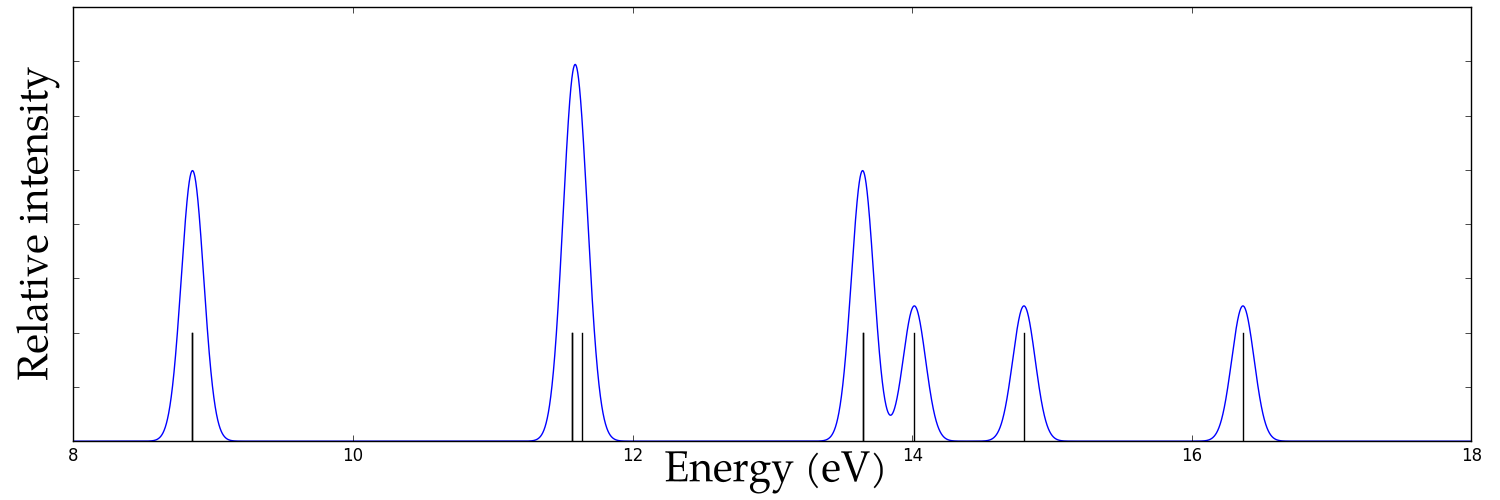
\includegraphics[width=0.9\textwidth]{zz_peaks.png}
    \end{figure}
    \pause
    \begin{figure}[h!]
        \centering
        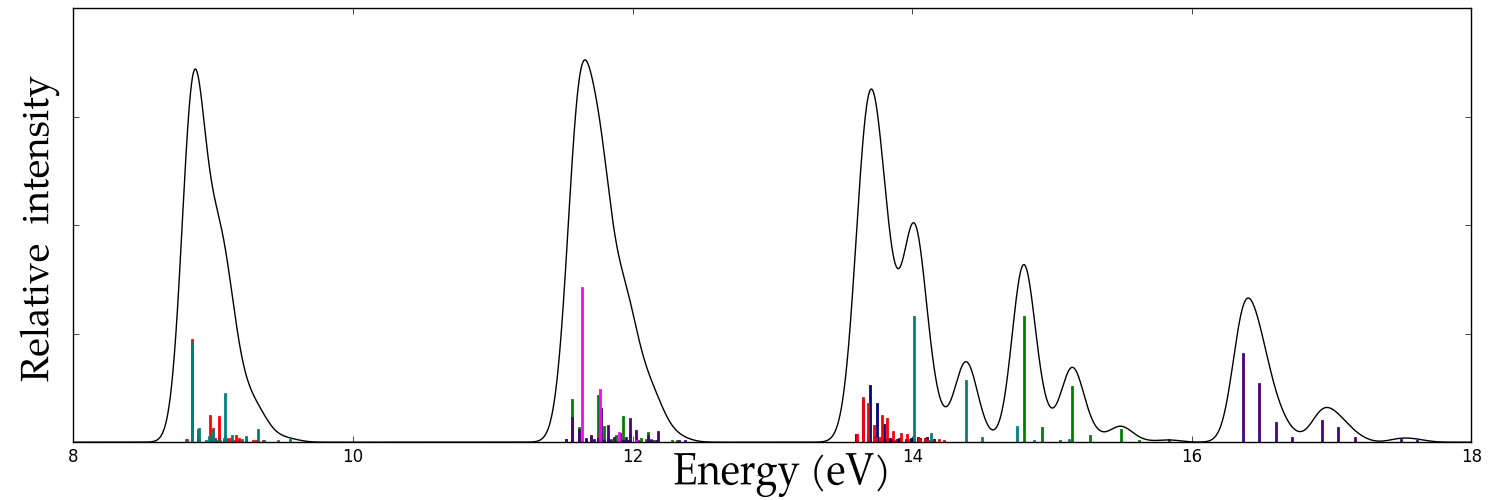
\includegraphics[width=0.9\textwidth]{all_peaks.png}
    \end{figure}
\end{frame}


% Is this needed??
\begin{frame}
    \frametitle{Electronic transition}
    \begin{overlayarea}{\textwidth}{14cm}
        \only<1>{
            \begin{figure}[h!]
                \centering
                \begin{subfigure}[b]{0.45\linewidth}
                    \caption*{Ground state}
                    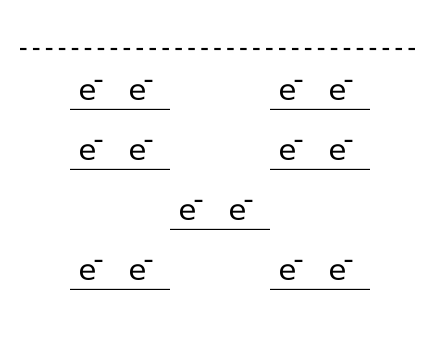
\includegraphics[width=\linewidth]{ele_full.png}
                \end{subfigure}
                \begin{subfigure}[b]{0.45\linewidth}
                    \caption*{Exited state}
                    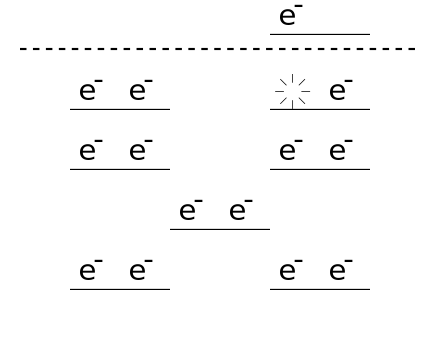
\includegraphics[width=\linewidth]{ele_ex1.png}
                \end{subfigure}
                %\caption{}
            \end{figure}
        }
        \only<2>{
            \begin{figure}[h!]
                \centering
                \begin{subfigure}[b]{0.45\linewidth}
                    \caption*{Ground state}
                    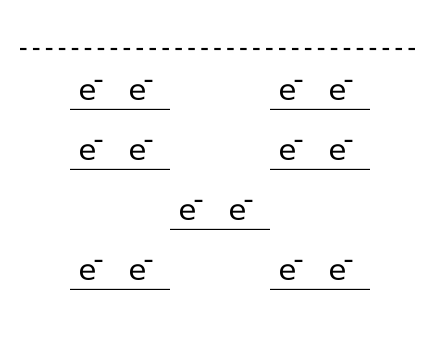
\includegraphics[width=\linewidth]{ele_full.png}
                \end{subfigure}
                \begin{subfigure}[b]{0.45\linewidth}
                    \caption*{Exited state}
                    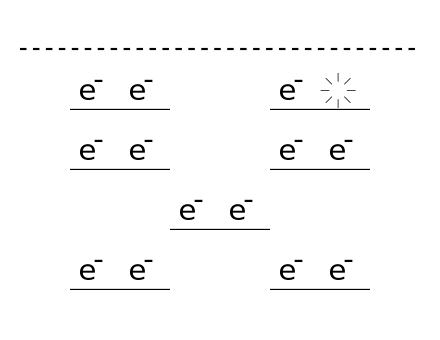
\includegraphics[width=\linewidth]{ele_ion_1.png}
                \end{subfigure}
                %\caption{}
            \end{figure}
        }
    \end{overlayarea}
\end{frame}


\begin{frame}
    \frametitle{Quantum harmonic oscillator}
        \only<2->{
            \begin{picture}(0, 0)
            \put(160, -135){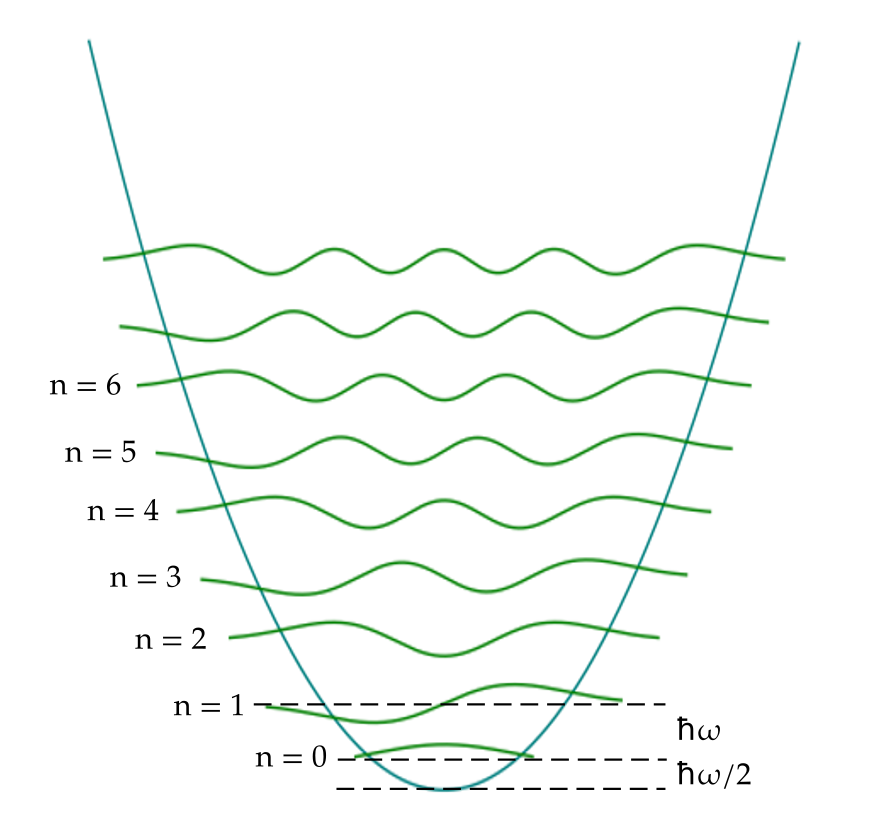
\includegraphics[width=6cm]{levels.png}}
            \end{picture}
        }
        \begin{align}
            &\hat{H} = \frac{\hbar}{2\mu} \pdv[2]{}{x} + {\underbrace{\textstyle \frac{1}{2} k \hat{x}^2}_{\mathclap{\text{Harmonic potential}}}} \nonumber \\
            &\hat{H}\ket{\psi} = E \ket{\psi} \nonumber
        \end{align}
        \pause
        After solving 
        \begin{align}
            &E_n = \hbar \omega \left(n +\frac{1}{2}\right) \nonumber \\
            &\psi_n(x) = \frac{1}{\sqrt{2^n n!}} \left(\frac{\mu \omega}{\pi \hbar}\right)^{1/4} e^{-\frac{\mu \omega x^2}{2 \hbar}} H_n\left( \sqrt{\frac{\mu \omega}{\hbar} x}\right) \nonumber
        \end{align}

\end{frame}


\begin{frame}
    \frametitle{Diatomic molecules}
    
    \begin{overlayarea}{\textwidth}{10cm}        
        \only<1>{
            \begin{wrapfigure}{r}{5.5cm}
                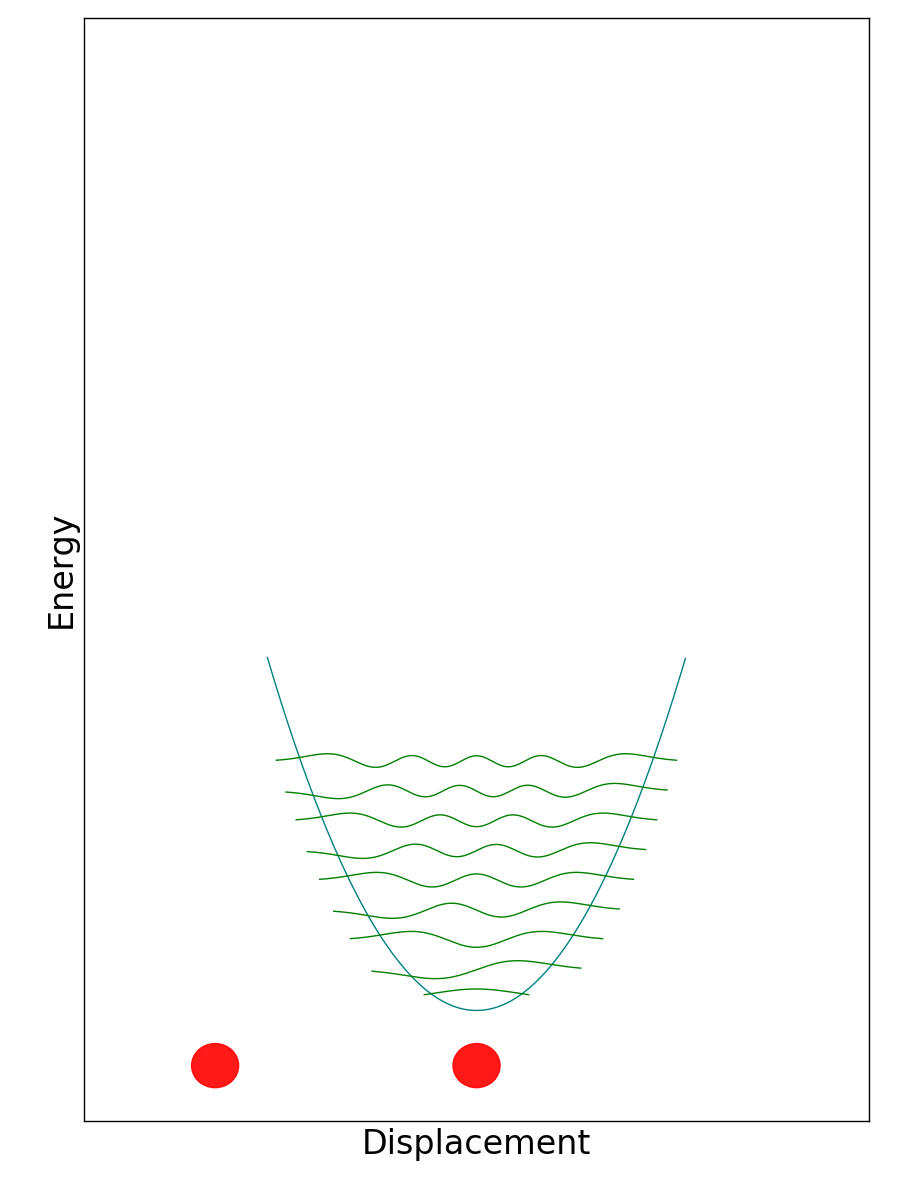
\includegraphics[width=5.5cm]{fc_build/step2.png}
            \end{wrapfigure}
            ~\\
            \mbox{Equilibrium distance $d$}
        }
        \only<2>{
            \begin{wrapfigure}{r}{5.5cm}
                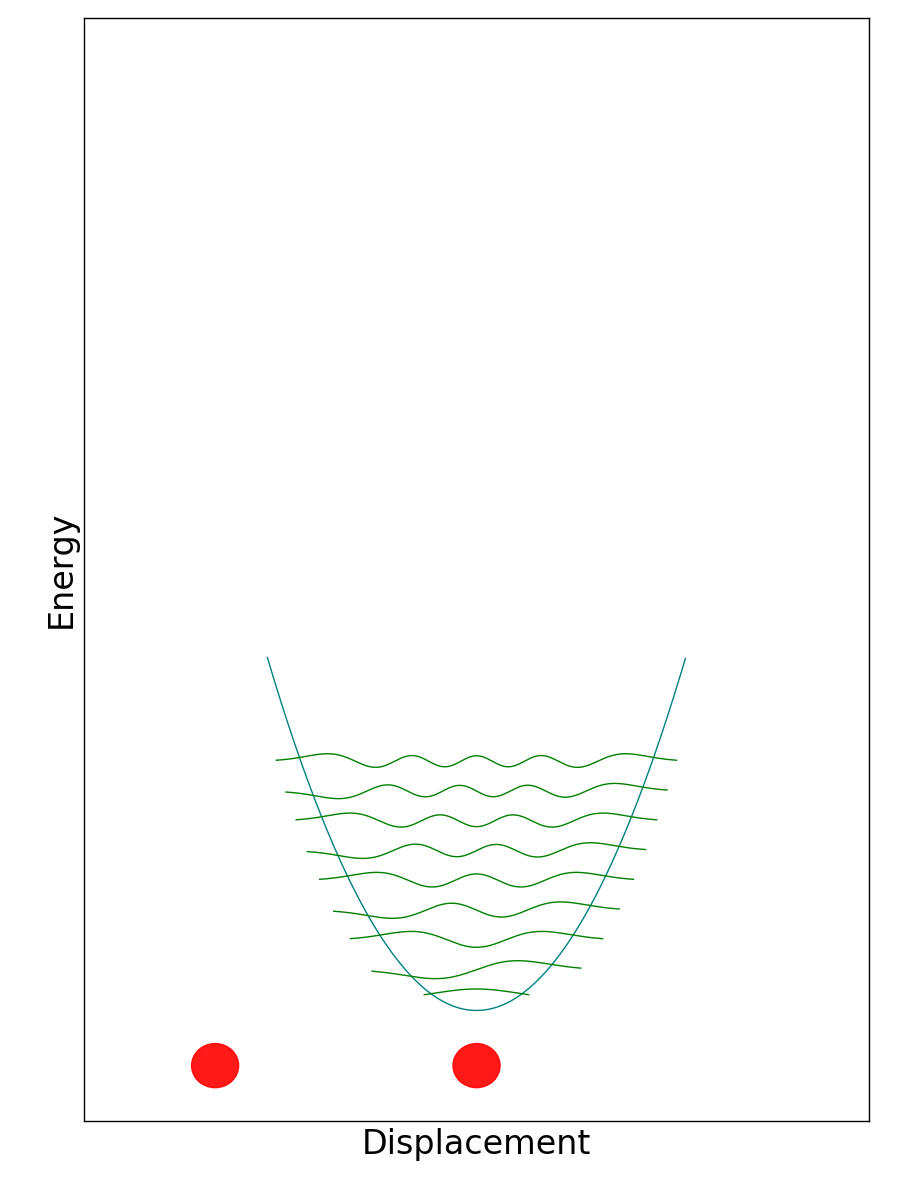
\includegraphics[width=5.5cm]{fc_build/step2.png}
            \end{wrapfigure}
            ~\\ 
            Equilibrium distance $d$ \\
            Frequency $\omega$ \\
            Force constant $k$ \\
            \mbox{Reduced mass $\mu$} \\
        }
        \only<3>{
            \begin{wrapfigure}{r}{5.5cm}
                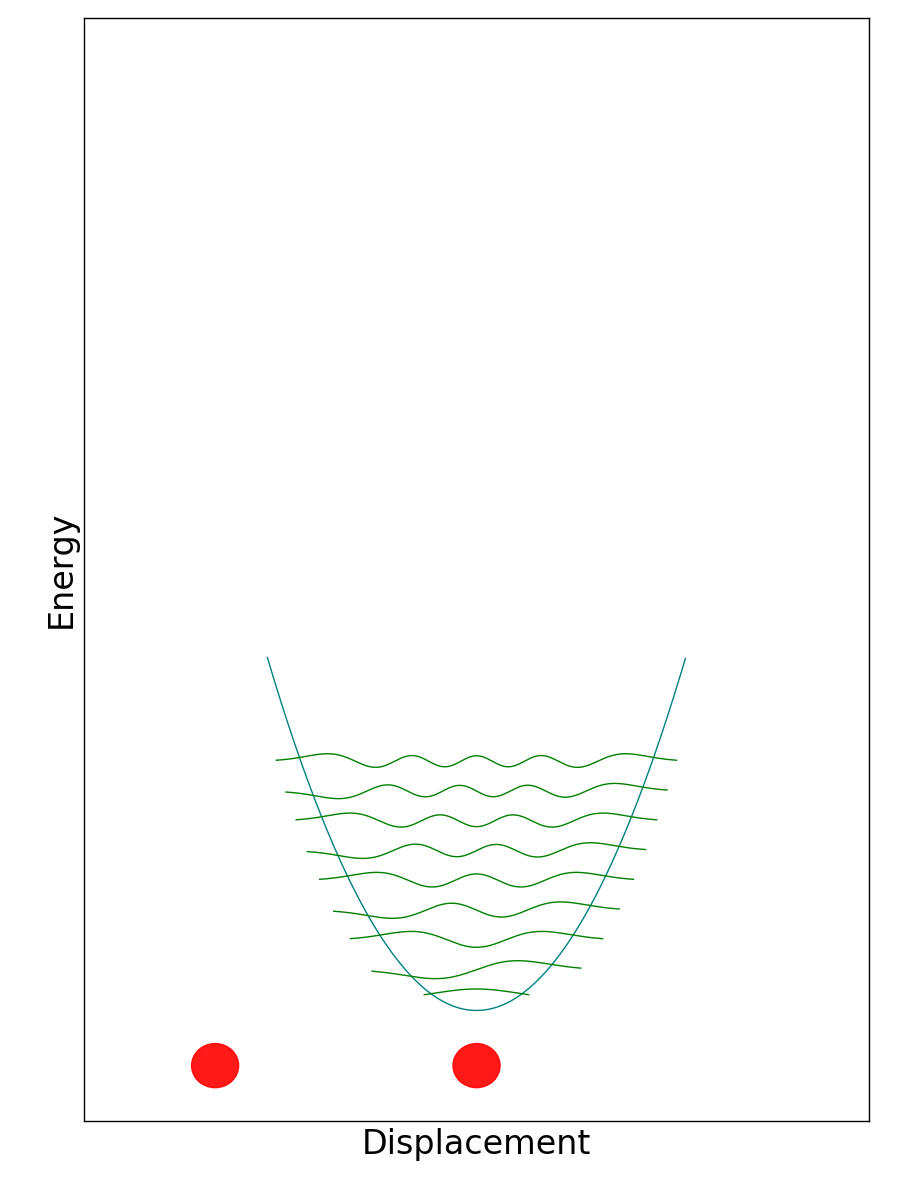
\includegraphics[width=5.5cm]{fc_build/step2.png}
            \end{wrapfigure}
            ~\\ 
            Equilibrium distance $d$ \\
            Frequency $\omega$ \\
            Force constant $k$ \\
            \mbox{Reduced mass $\mu$} \\
            Energy $E_n = \hbar \omega (n+\frac{1}{2})$ \\
        }
        \only<4>{
            \begin{wrapfigure}{r}{5.5cm}
                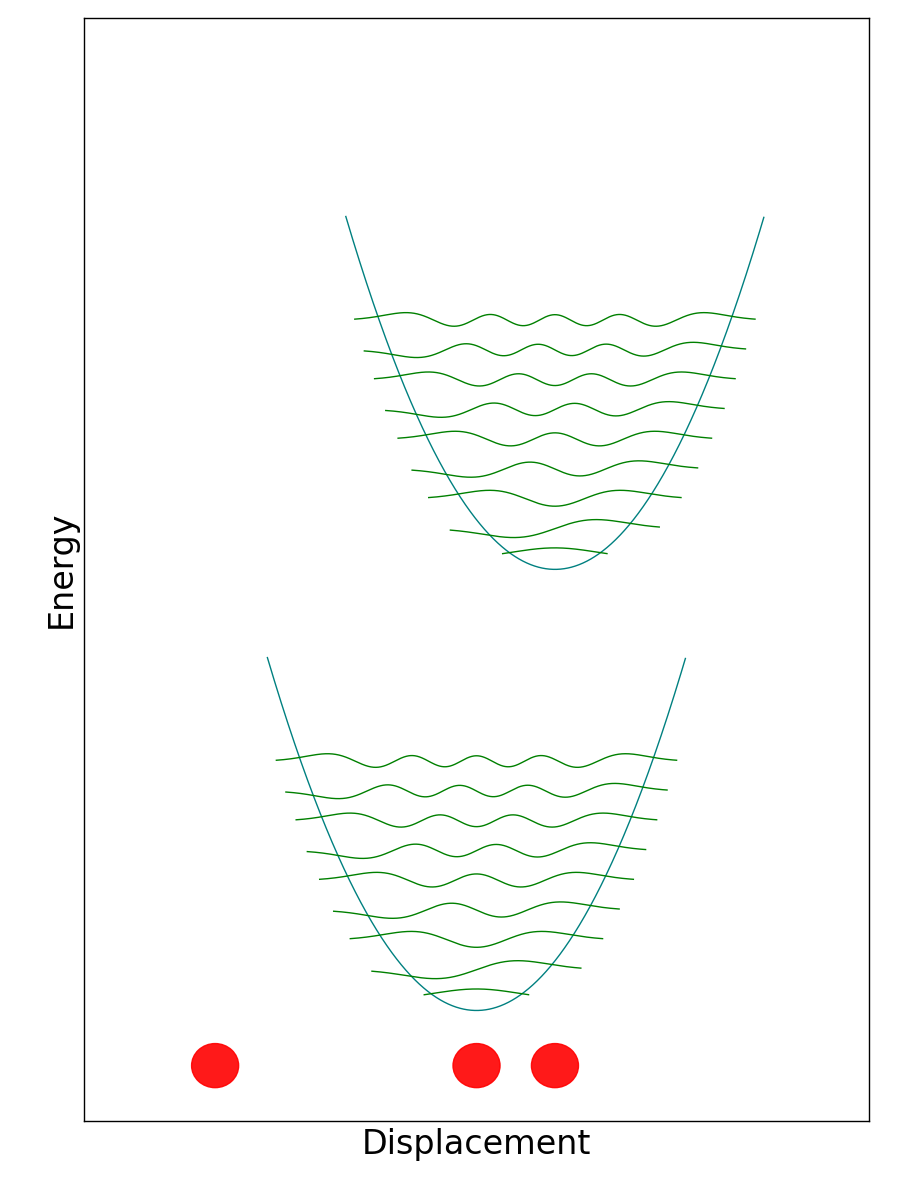
\includegraphics[width=5.5cm]{fc_build/step5.png}
            \end{wrapfigure}
            ~\\ 
            Equilibrium distance $d$ \\
            Frequency $\omega$ \\
            Force constant $k$ \\
            \mbox{Reduced mass $\mu$} \\
            Energy $E_n = \hbar \omega (n+\frac{1}{2})$ \\
            Equilibrium distance $d'$ \\
            Energy $E_{n'} = \hbar \omega (n'+\frac{1}{2})$ \\
        }
        \only<5>{
            \begin{wrapfigure}{r}{5.5cm}
                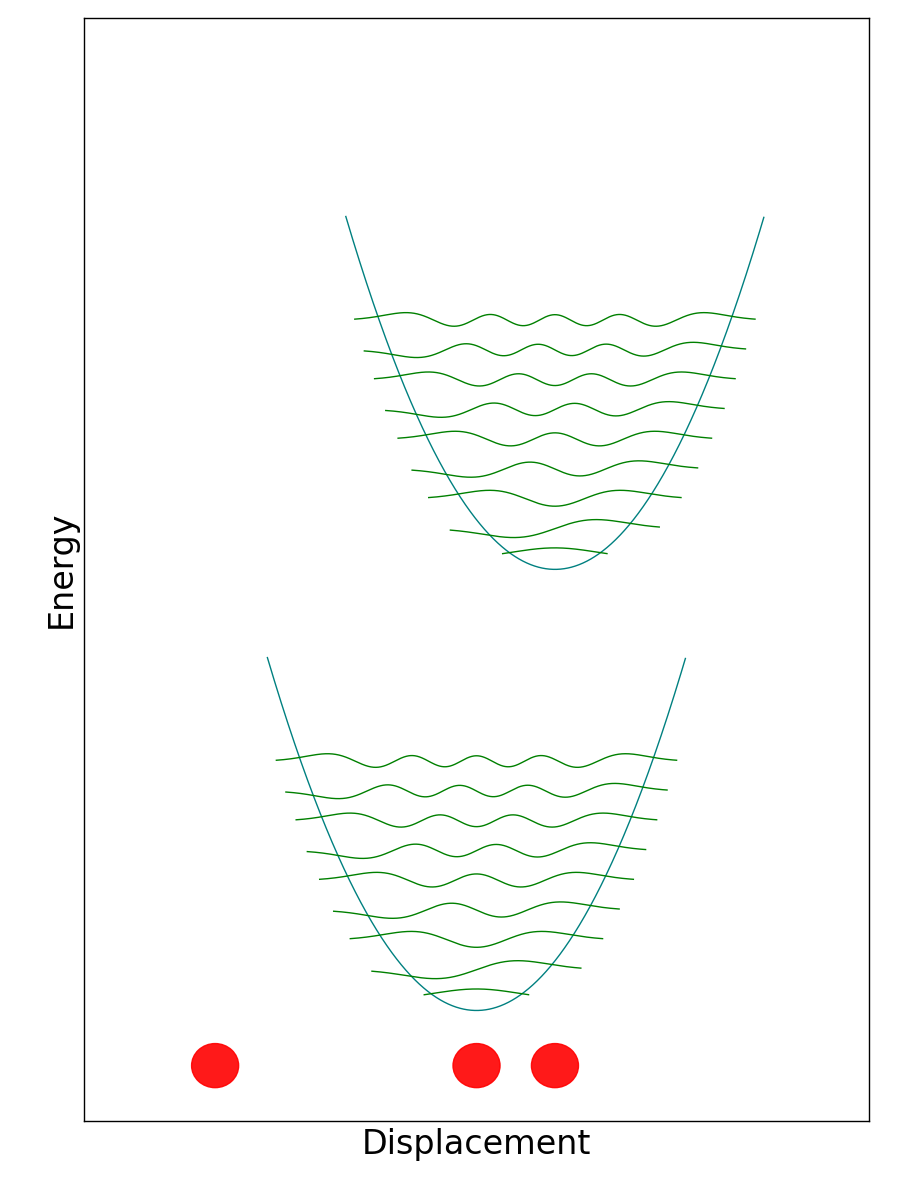
\includegraphics[width=5.5cm]{fc_build/step5.png}
            \end{wrapfigure}
            ~\\ 
            Equilibrium distance $d$ \\
            Frequency $\omega$ \\
            Force constant $k$ \\
            \mbox{Reduced mass $\mu$} \\
            Energy $E_n = \hbar \omega (n+\frac{1}{2})$ \\
            Equilibrium distance $d'$ \\
            Energy $E_{n'} = \hbar \omega (n'+\frac{1}{2})$ \\
            Displacement $\delta = d'-d$
        }
        \only<6>{
            \begin{wrapfigure}{r}{5.5cm}
                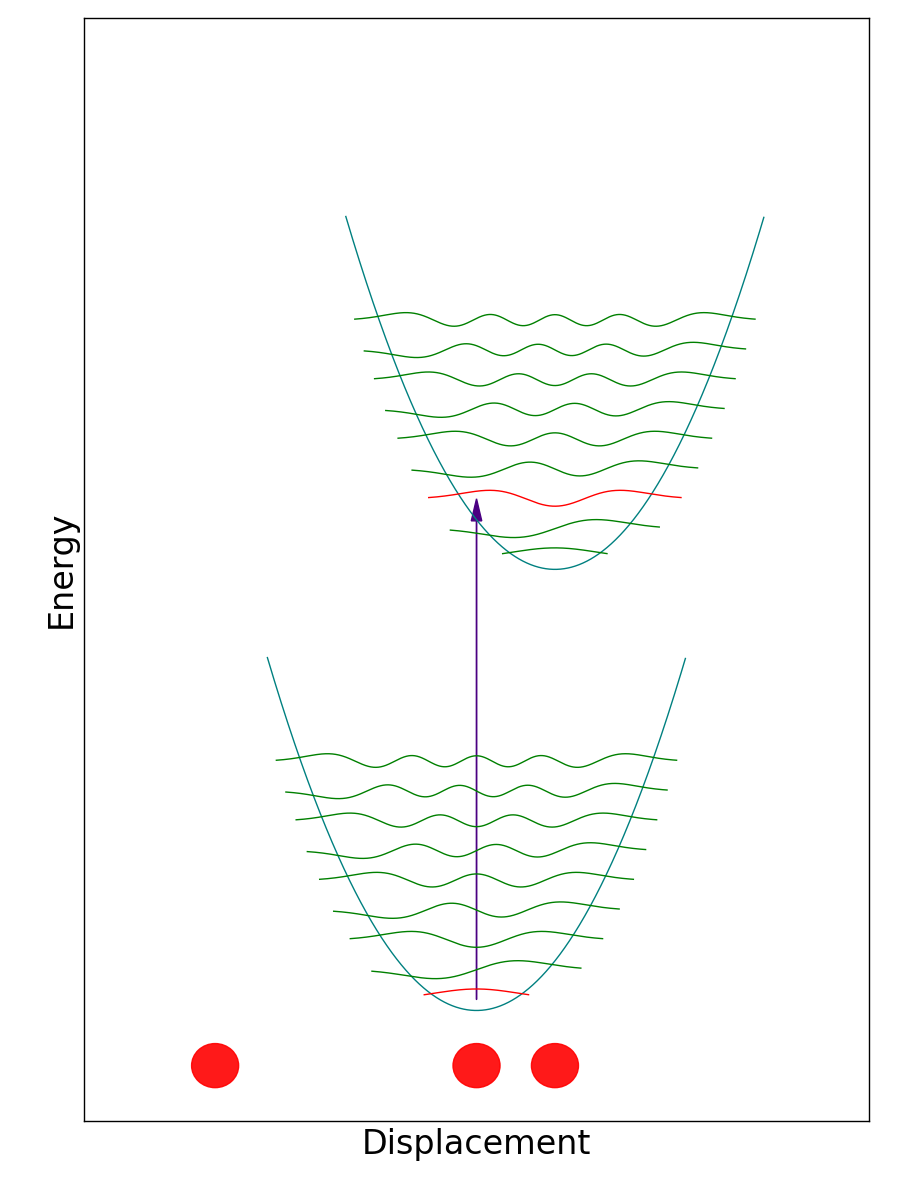
\includegraphics[width=5.5cm]{fc_build/step7.png}
            \end{wrapfigure}
            ~\\ 
            Equilibrium distance $d$ \\
            Frequency $\omega$ \\
            Force constant $k$ \\
            \mbox{Reduced mass $\mu$} \\
            Energy $E_n = \hbar \omega (n+\frac{1}{2})$ \\
            Equilibrium distance $d'$ \\
            Energy $E_{n'} = \hbar \omega (n'+\frac{1}{2})$ \\
            Displacement $\delta = d'-d$ \\ 
            \begin{align}
            \mathrm{I}_{n \to n'} &= \abs{\braket{\psi^{\ast}_{final}}{\psi^{}_{initial}}}^2 \nonumber \\
                                  &= \mathrm{FCI}(n,n')^2 \nonumber 
            \end{align}
        }
    \end{overlayarea}
\end{frame}

\begin{frame}
    \frametitle{Transitions for diatomic molecule}
    \begin{overlayarea}{\textwidth}{14cm}
        \only<1>{
            \begin{figure}[h!]
                \centering
                \begin{subfigure}[b]{0.45\linewidth}
                    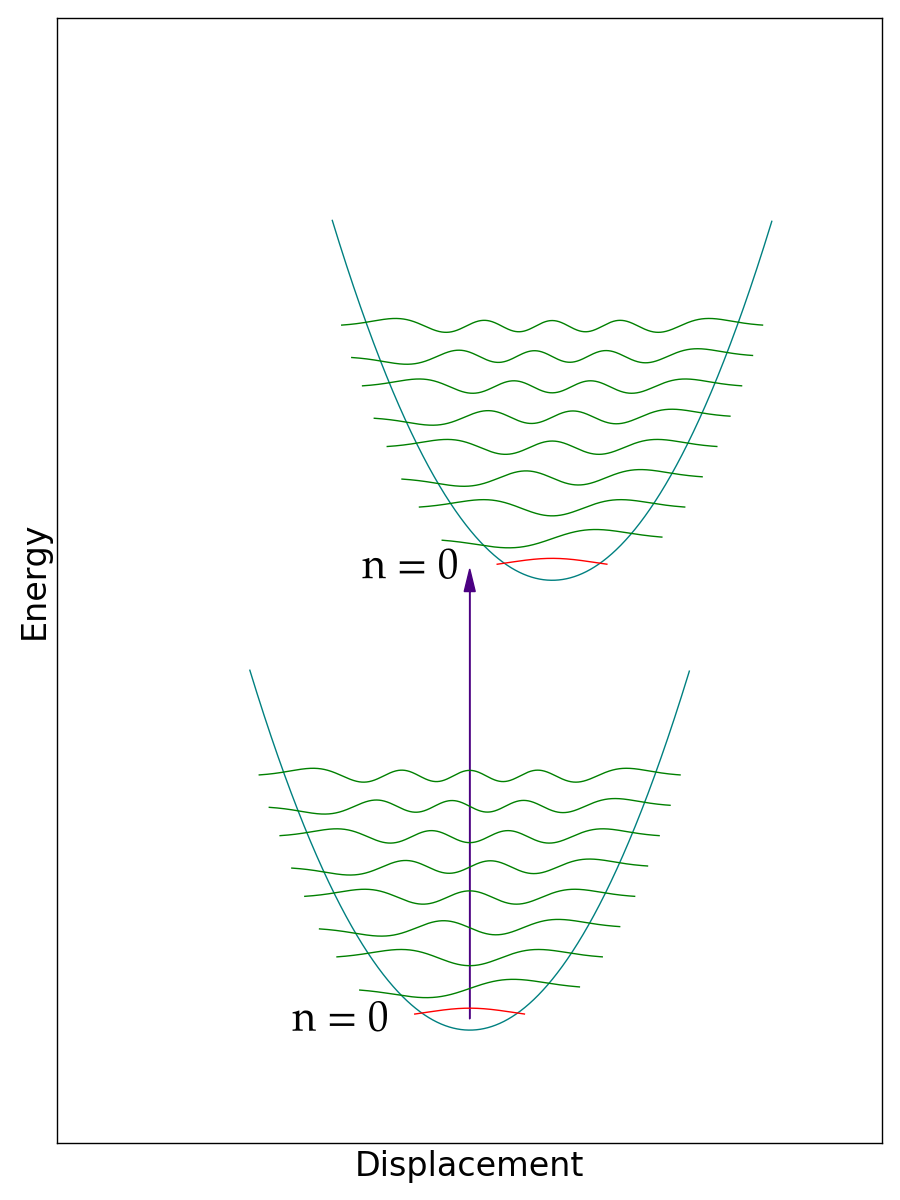
\includegraphics[width=\linewidth]{fc/tr_0.png}
                \end{subfigure}
                \begin{subfigure}[b]{0.45\linewidth}
                    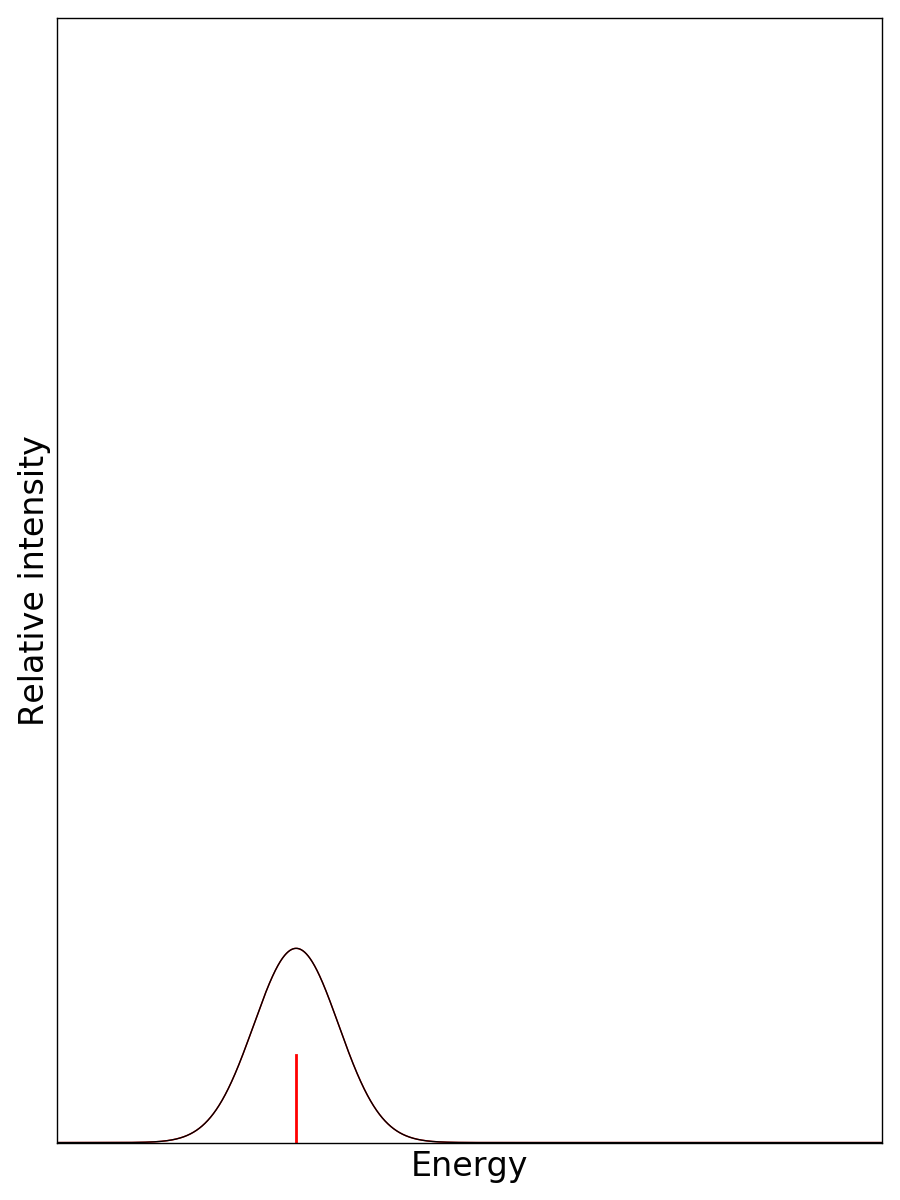
\includegraphics[width=\linewidth]{fc_sp/sp_0.png}
                \end{subfigure}
                %\caption{}
            \end{figure}
        }
        \only<2>{
            \begin{figure}[h!]
                \centering
                \begin{subfigure}[b]{0.45\linewidth}
                    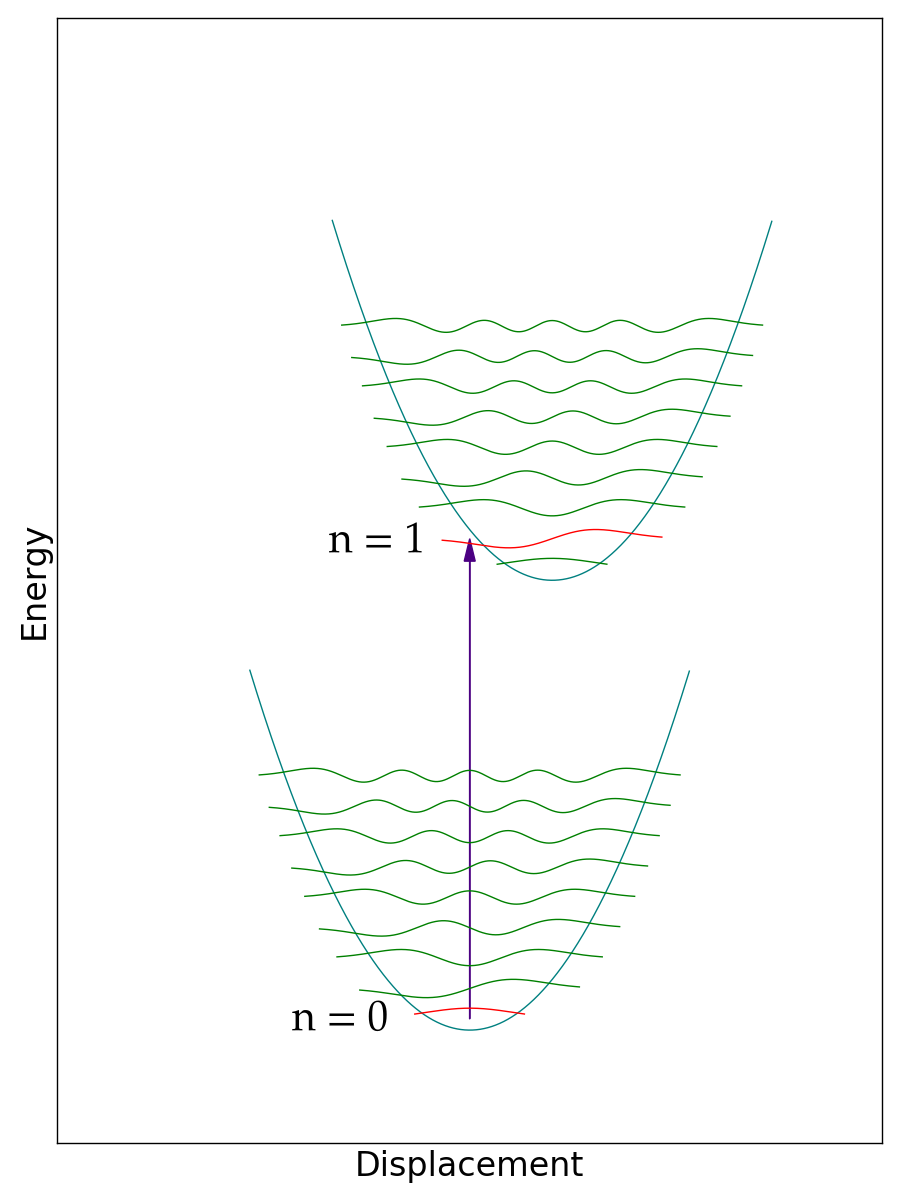
\includegraphics[width=\linewidth]{fc/tr_1.png}
                \end{subfigure}
                \begin{subfigure}[b]{0.45\linewidth}
                    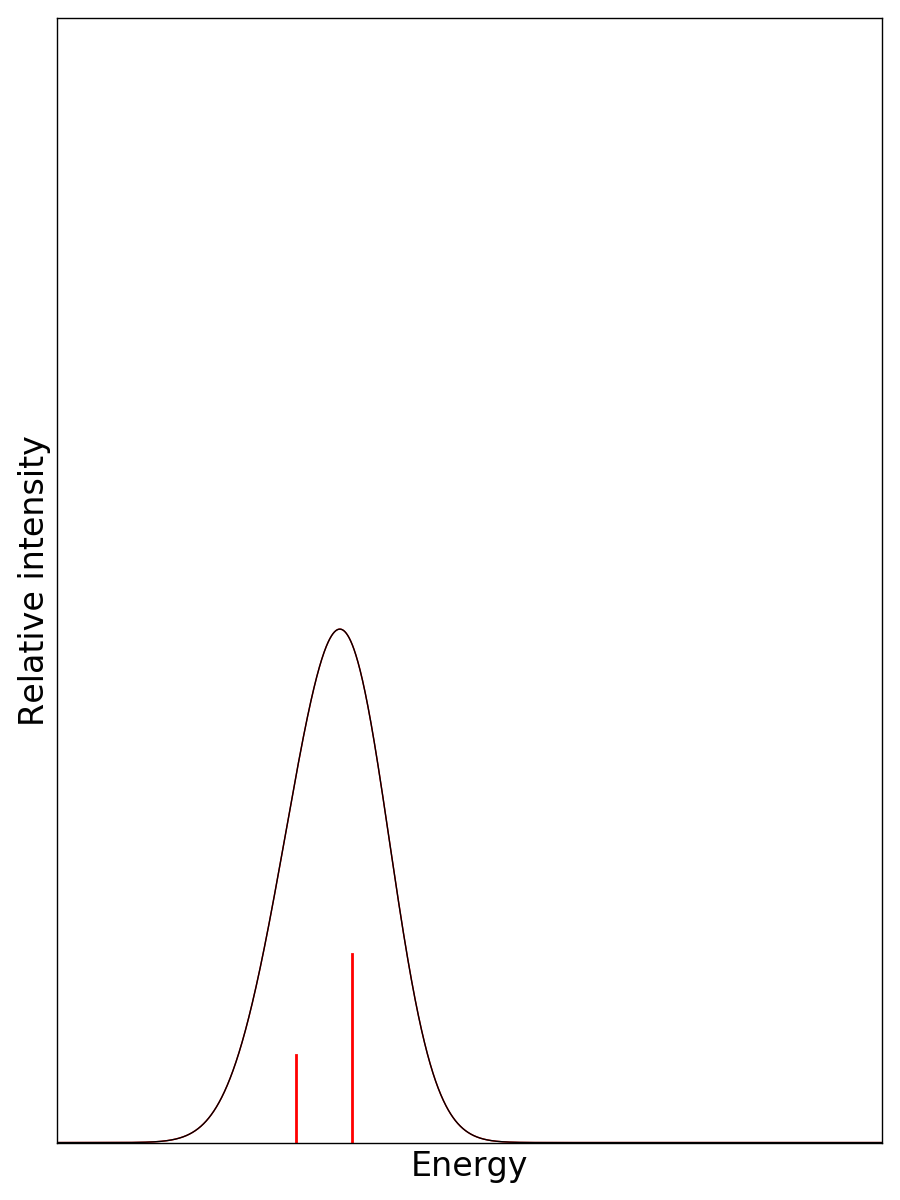
\includegraphics[width=\linewidth]{fc_sp/sp_1.png}
                \end{subfigure}
                %\caption{}
            \end{figure}
        }
        \only<3>{
            \begin{figure}[h!]
                \centering
                \begin{subfigure}[b]{0.45\linewidth}
                    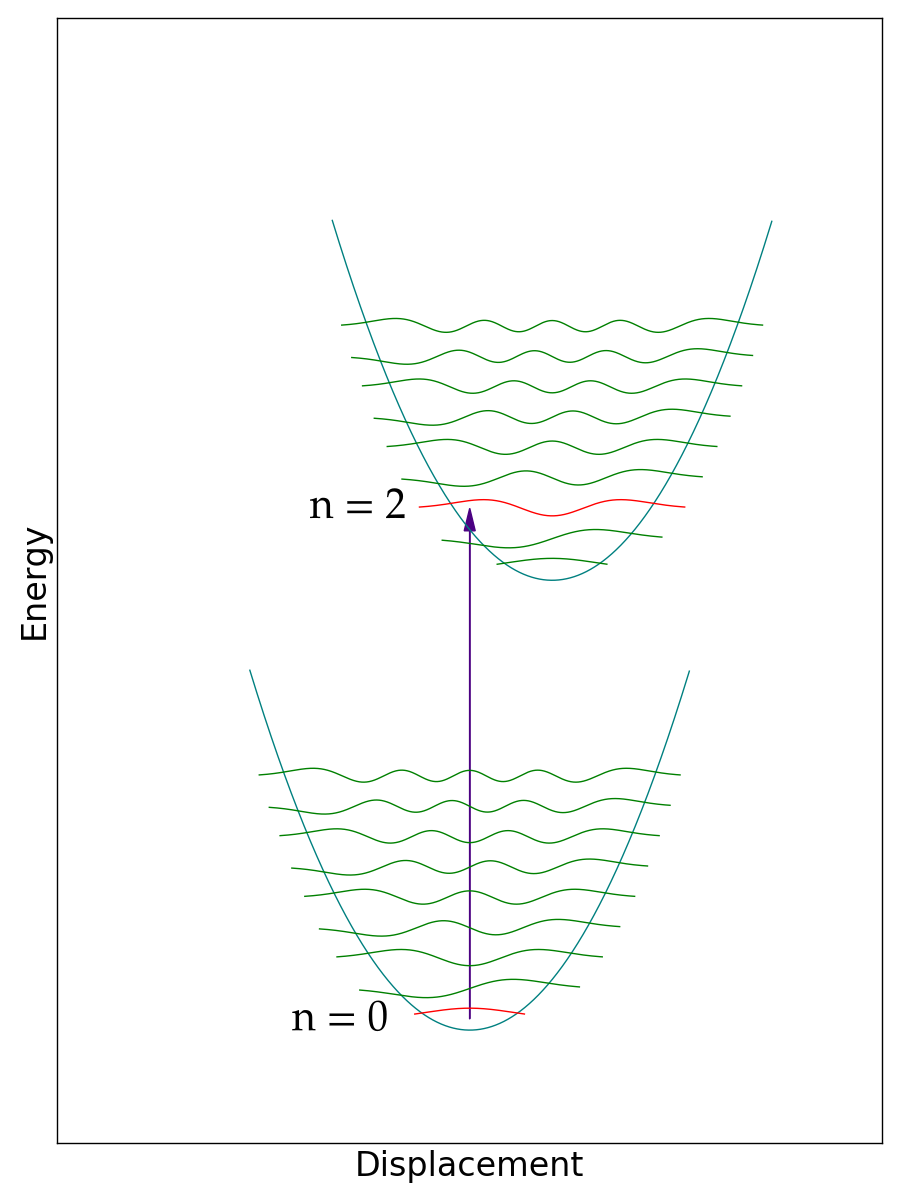
\includegraphics[width=\linewidth]{fc/tr_2.png}
                \end{subfigure}
                \begin{subfigure}[b]{0.45\linewidth}
                    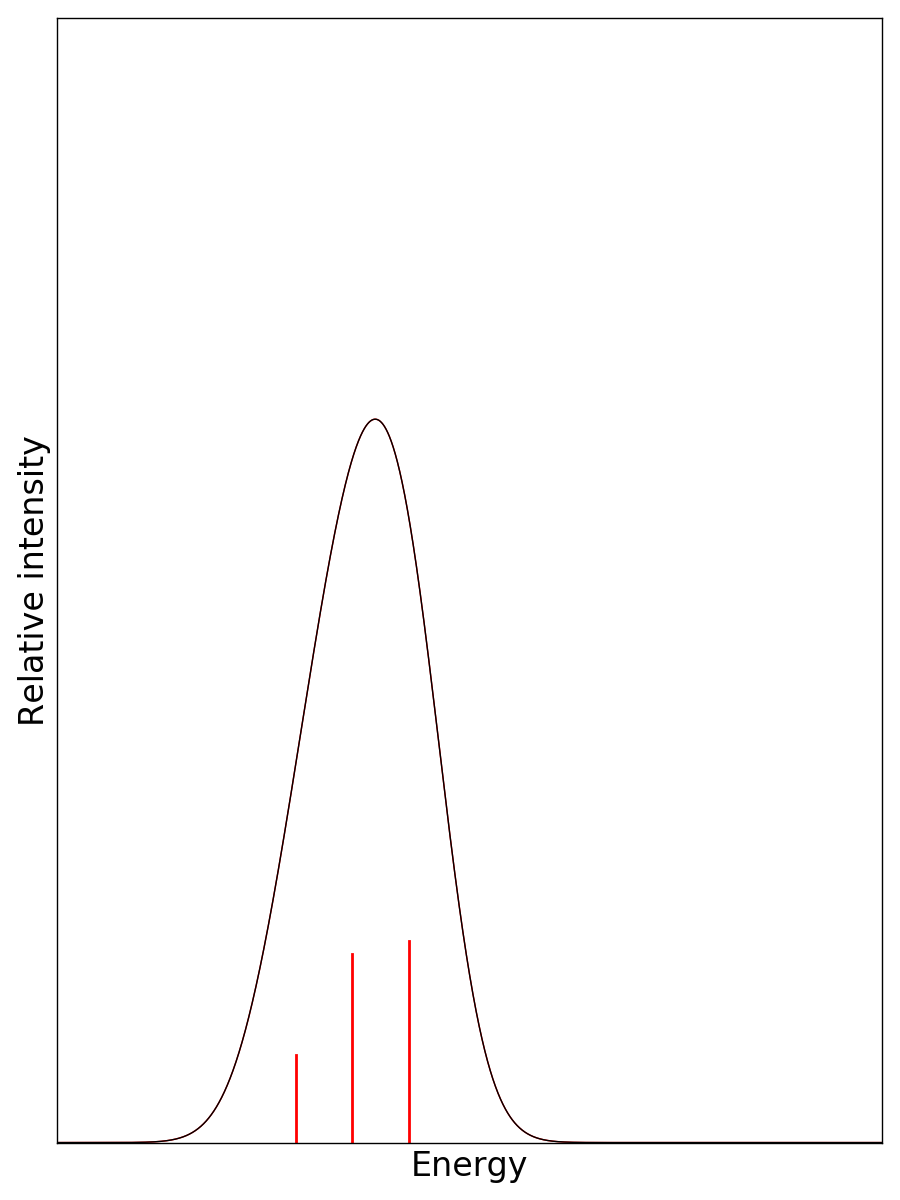
\includegraphics[width=\linewidth]{fc_sp/sp_2.png}
                \end{subfigure}
                %\caption{}
            \end{figure}
        }
        \only<4>{
            \begin{figure}[h!]
                \centering
                \begin{subfigure}[b]{0.45\linewidth}
                    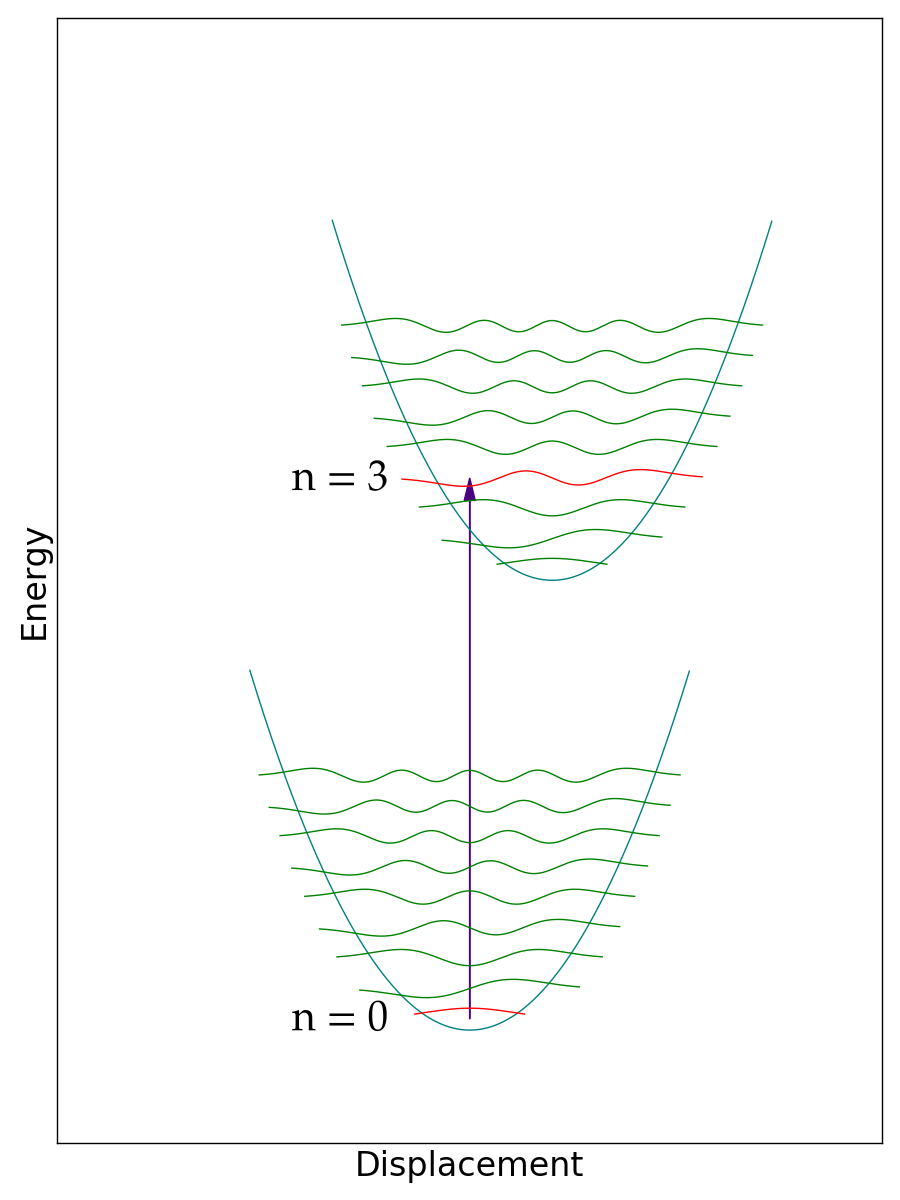
\includegraphics[width=\linewidth]{fc/tr_3.png}
                \end{subfigure}
                \begin{subfigure}[b]{0.45\linewidth}
                    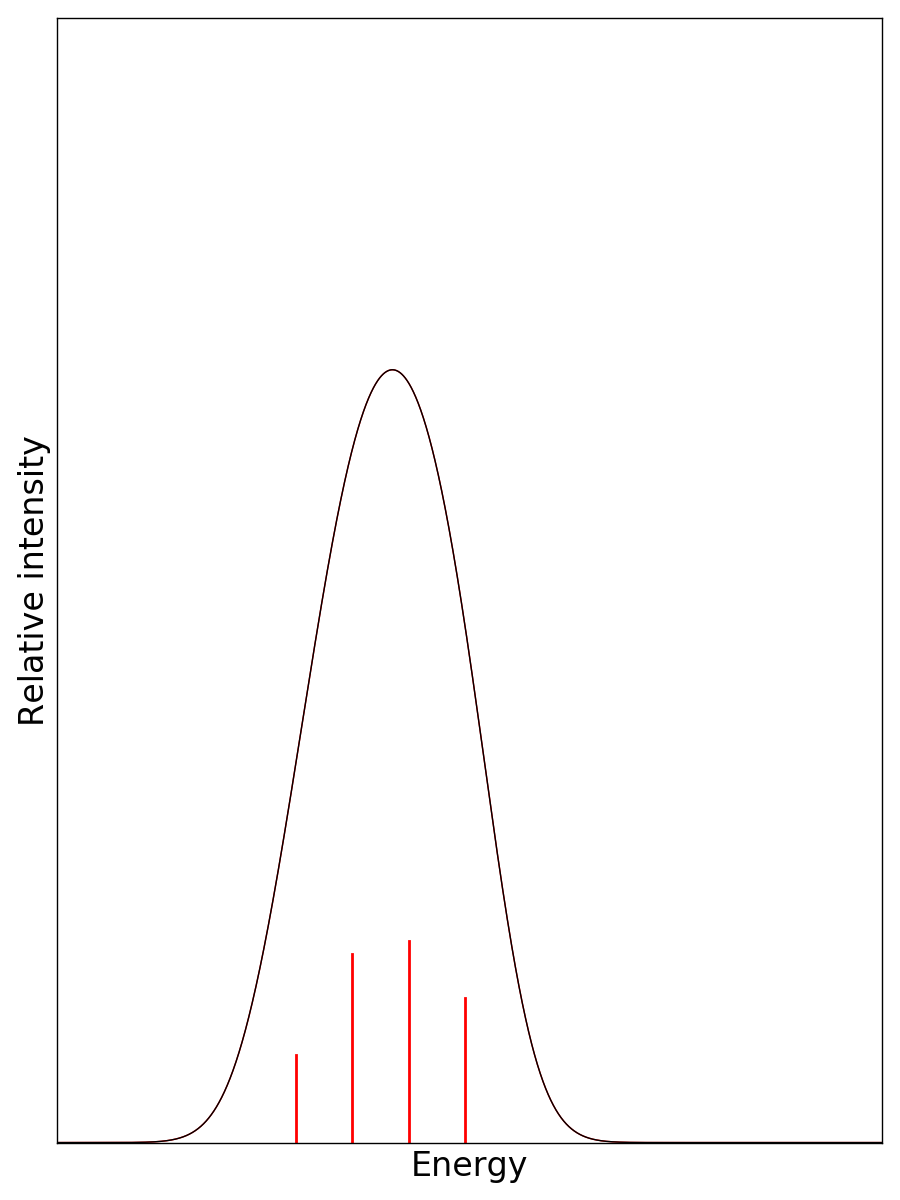
\includegraphics[width=\linewidth]{fc_sp/sp_3.png}
                \end{subfigure}
                %\caption{}
            \end{figure}
        }
        \only<5>{
            \begin{figure}[h!]
                \centering
                \begin{subfigure}[b]{0.45\linewidth}
                    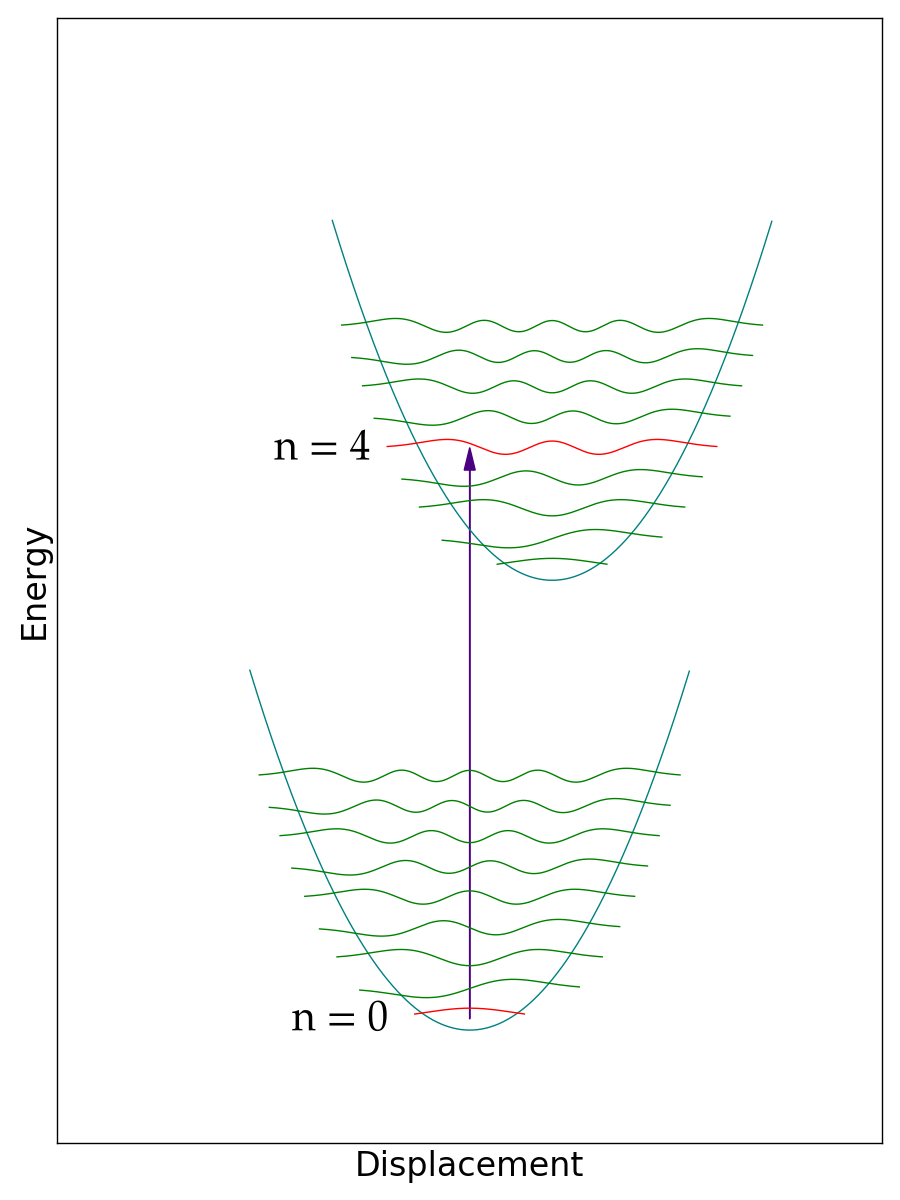
\includegraphics[width=\linewidth]{fc/tr_4.png}
                \end{subfigure}
                \begin{subfigure}[b]{0.45\linewidth}
                    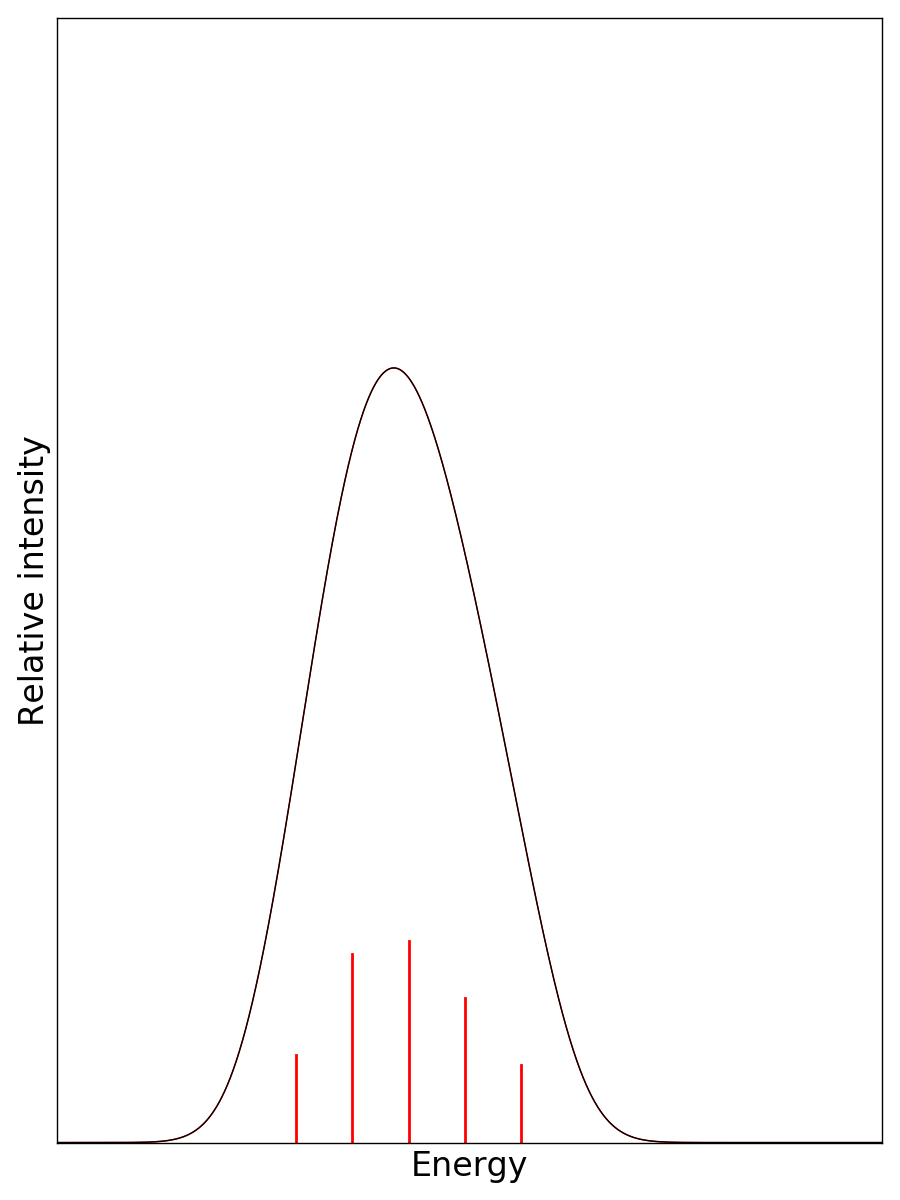
\includegraphics[width=\linewidth]{fc_sp/sp_4.png}
                \end{subfigure}
                %\caption{}
            \end{figure}
        }
        \only<6>{
            \begin{figure}[h!]
                \centering
                \begin{subfigure}[b]{0.45\linewidth}
                    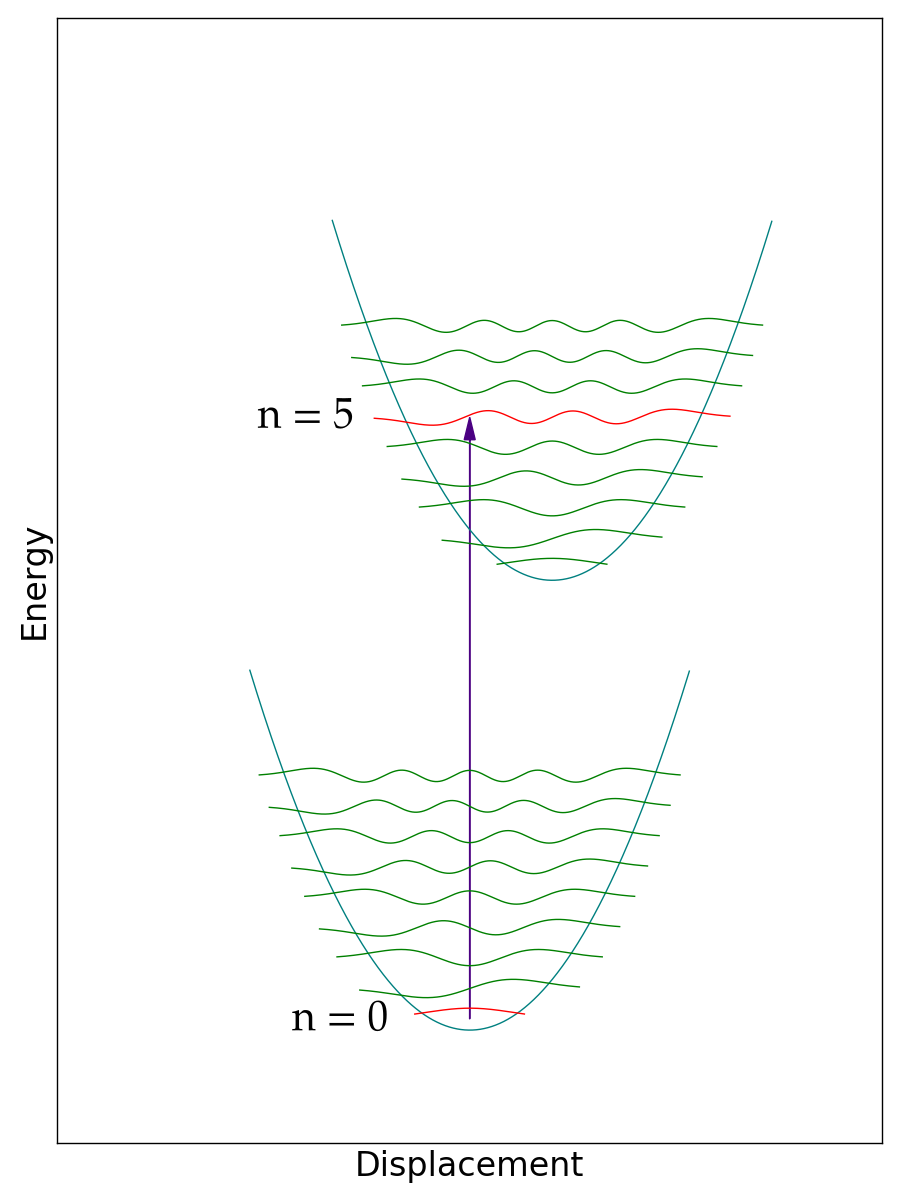
\includegraphics[width=\linewidth]{fc/tr_5.png}
                \end{subfigure}
                \begin{subfigure}[b]{0.45\linewidth}
                    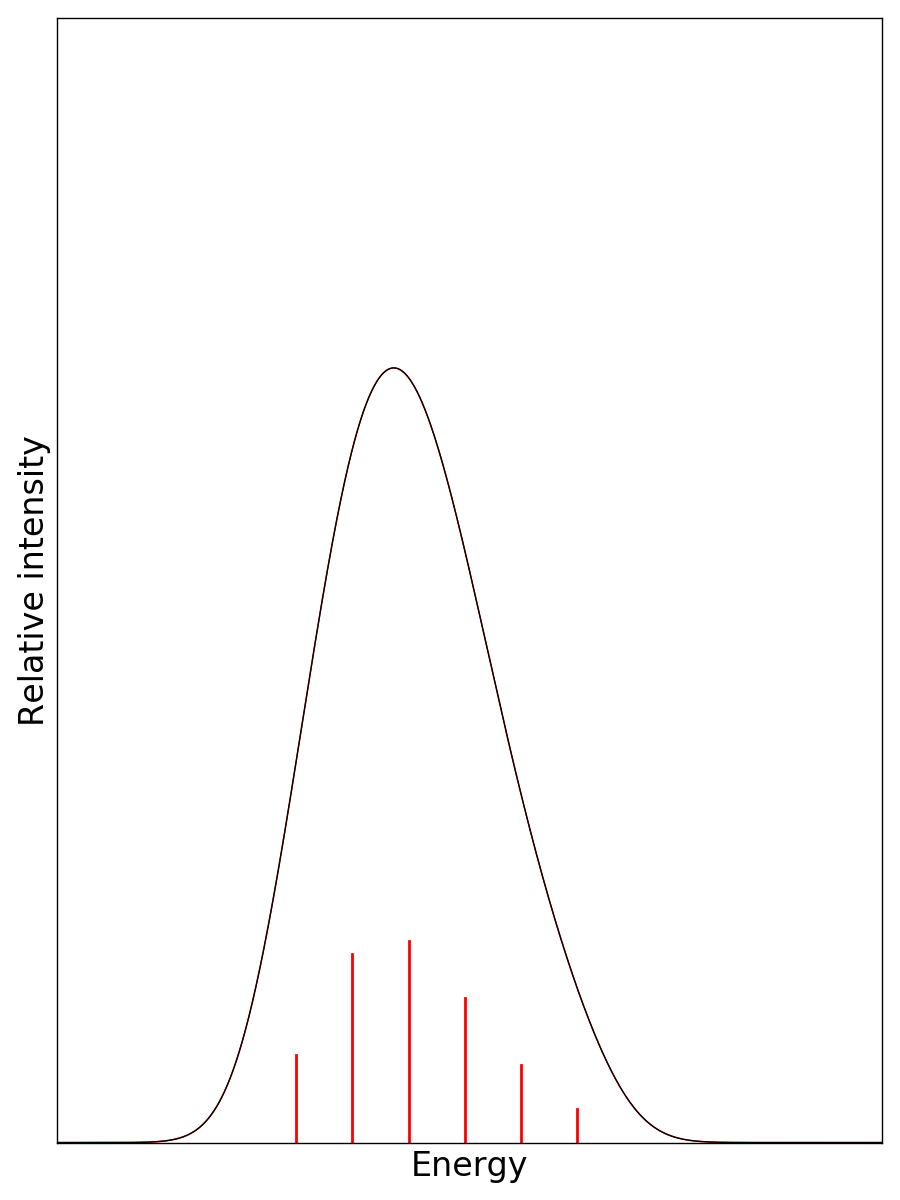
\includegraphics[width=\linewidth]{fc_sp/sp_5.png}
                \end{subfigure}
                %\caption{}
            \end{figure}
        }
        \only<7>{
            \begin{figure}[h!]
                \centering
                \begin{subfigure}[b]{0.45\linewidth}
                    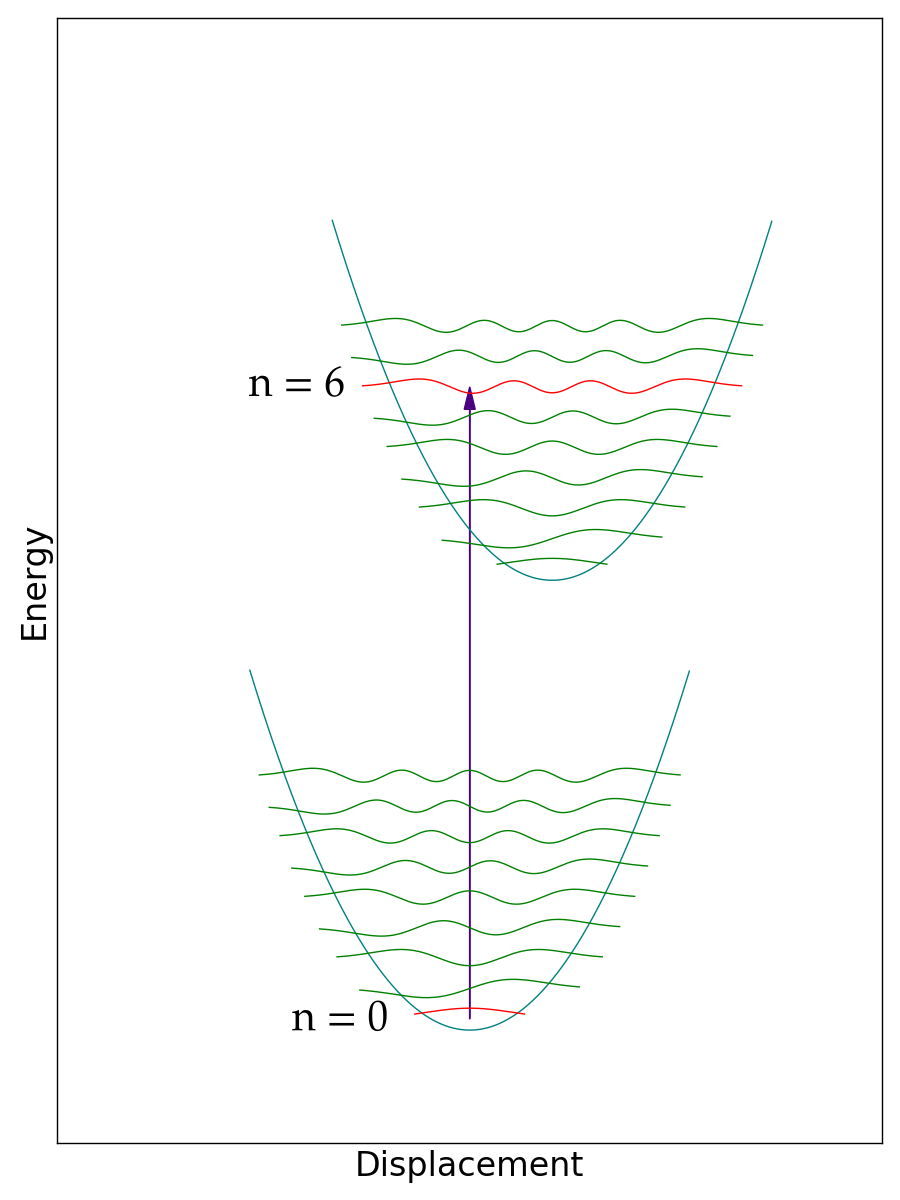
\includegraphics[width=\linewidth]{fc/tr_6.png}
                \end{subfigure}
                \begin{subfigure}[b]{0.45\linewidth}
                    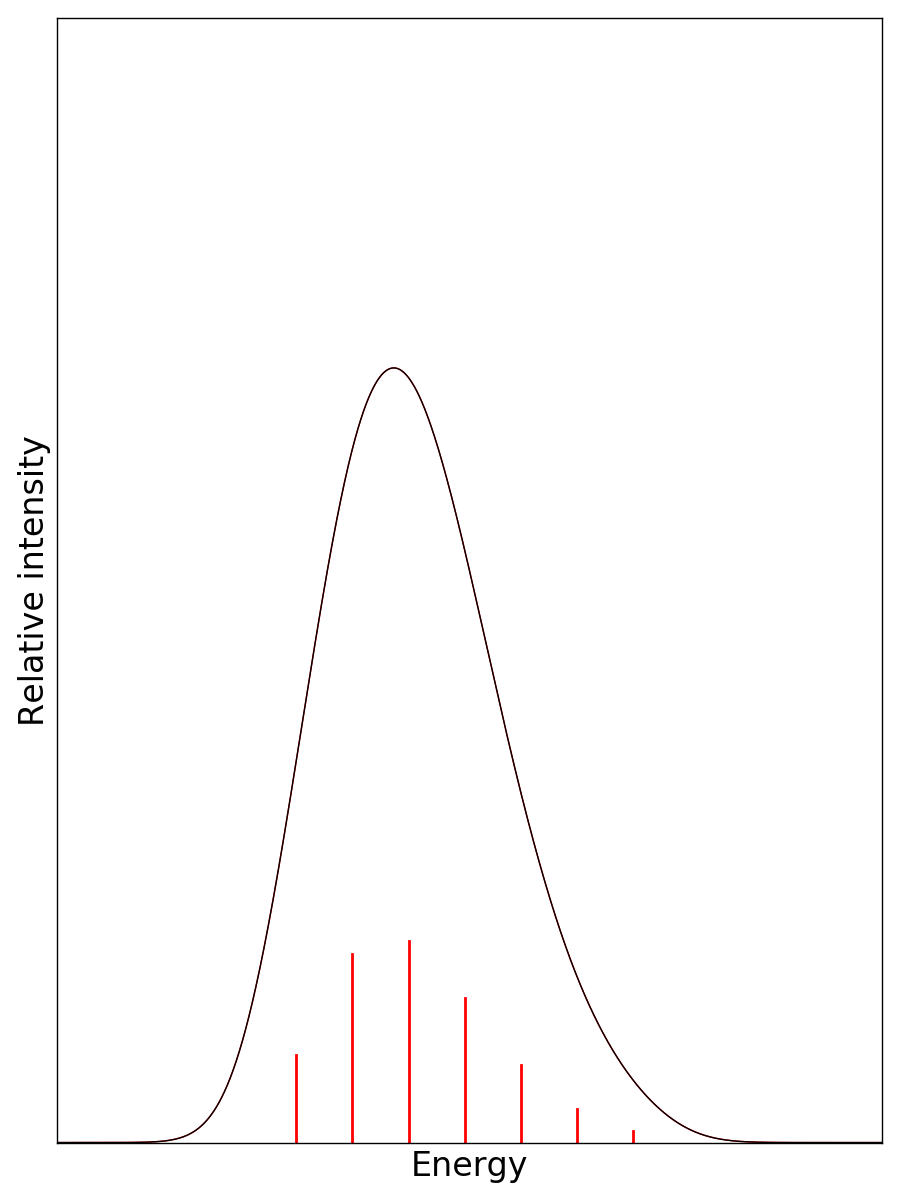
\includegraphics[width=\linewidth]{fc_sp/sp_6.png}
                \end{subfigure}
                %\caption{}
            \end{figure}
        }
        \only<8>{
            \begin{figure}[h!]
                \centering
                \begin{subfigure}[b]{0.45\linewidth}
                    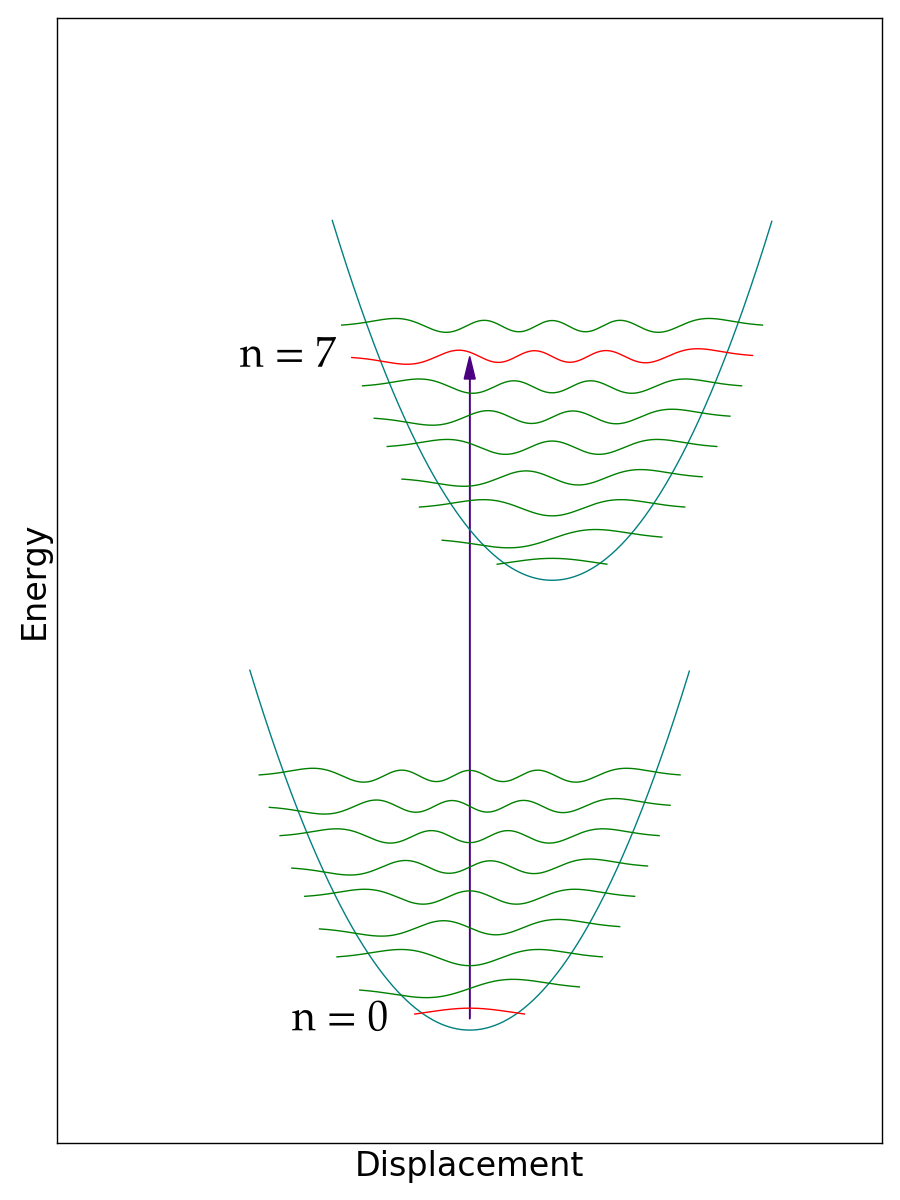
\includegraphics[width=\linewidth]{fc/tr_7.png}
                \end{subfigure}
                \begin{subfigure}[b]{0.45\linewidth}
                    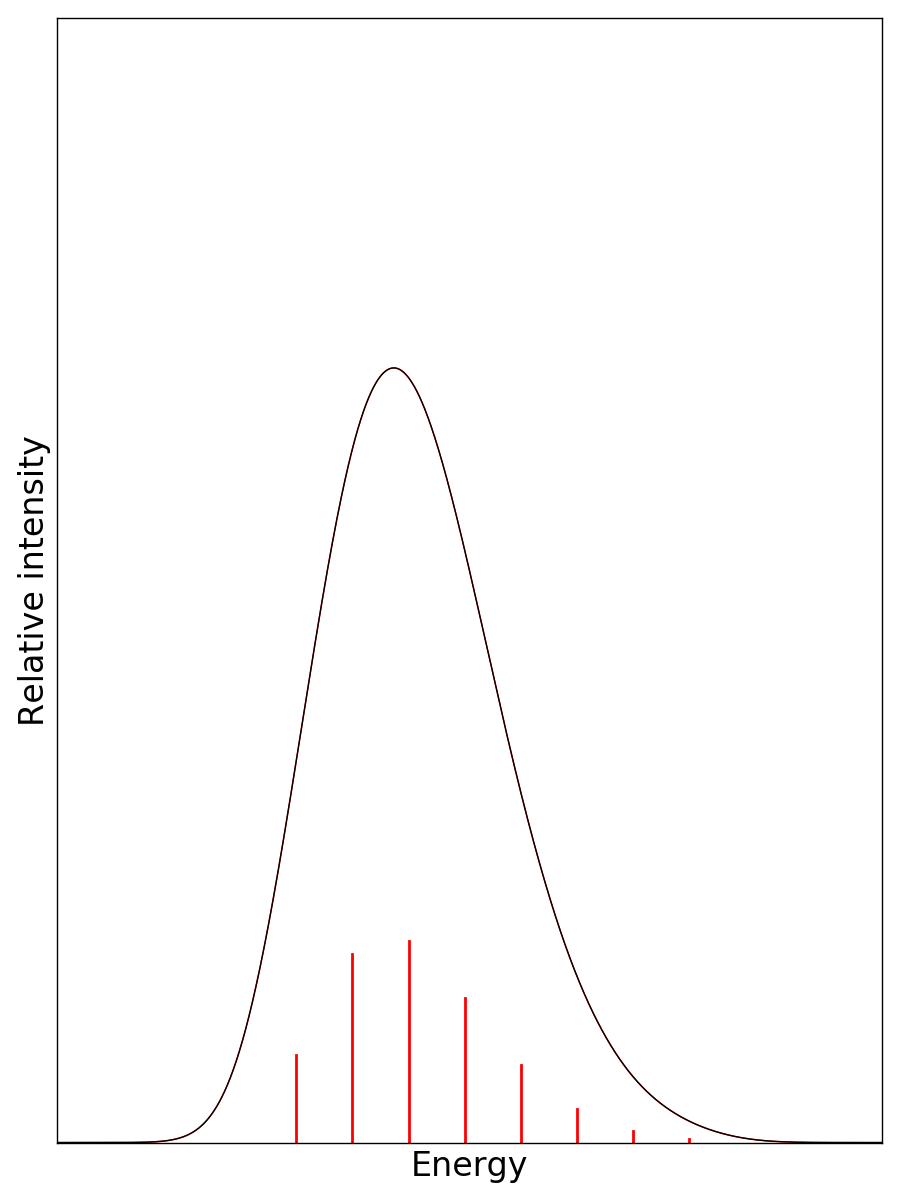
\includegraphics[width=\linewidth]{fc_sp/sp_7.png}
                \end{subfigure}
                %\caption{}
            \end{figure}
        }
        \only<9>{
            \begin{figure}[h!]
                \centering
                \begin{subfigure}[b]{0.45\linewidth}
                    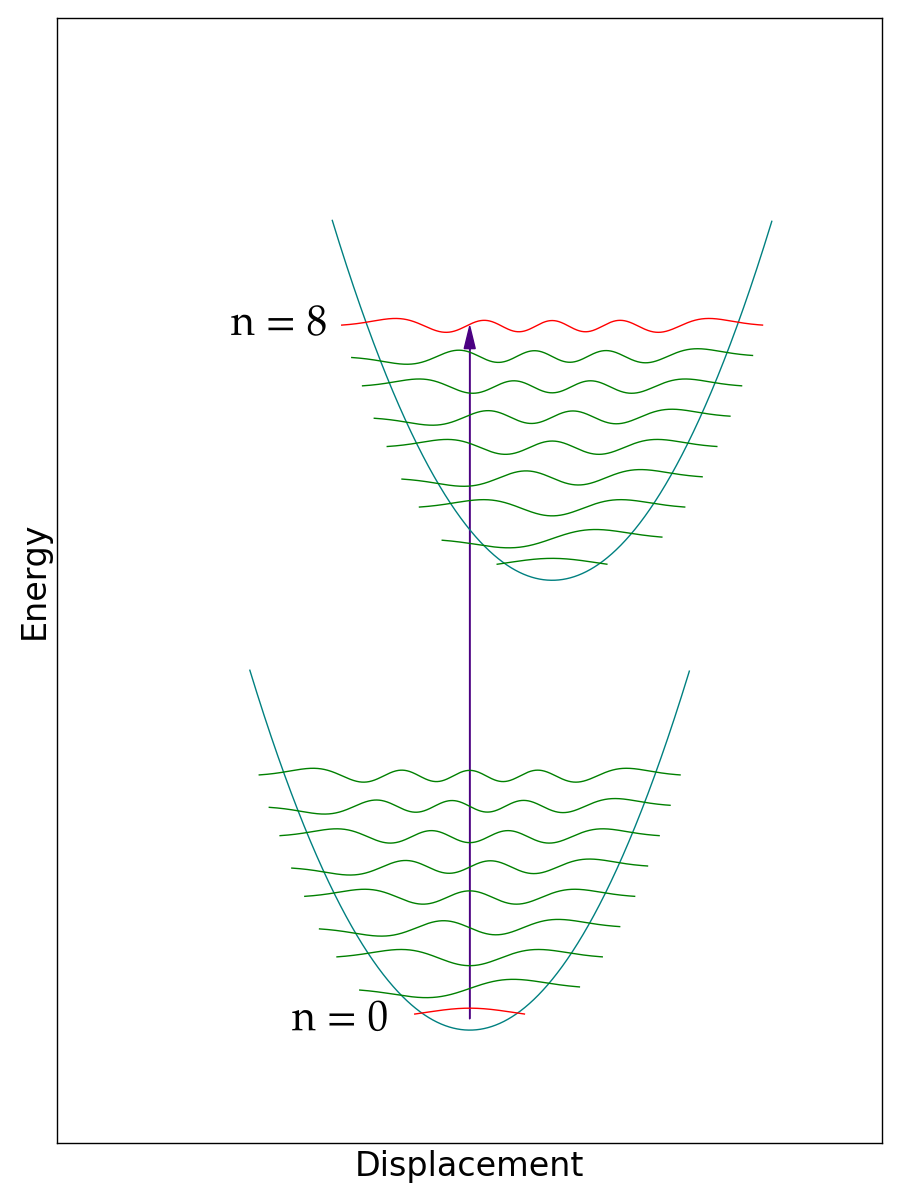
\includegraphics[width=\linewidth]{fc/tr_8.png}
                \end{subfigure}
                \begin{subfigure}[b]{0.45\linewidth}
                    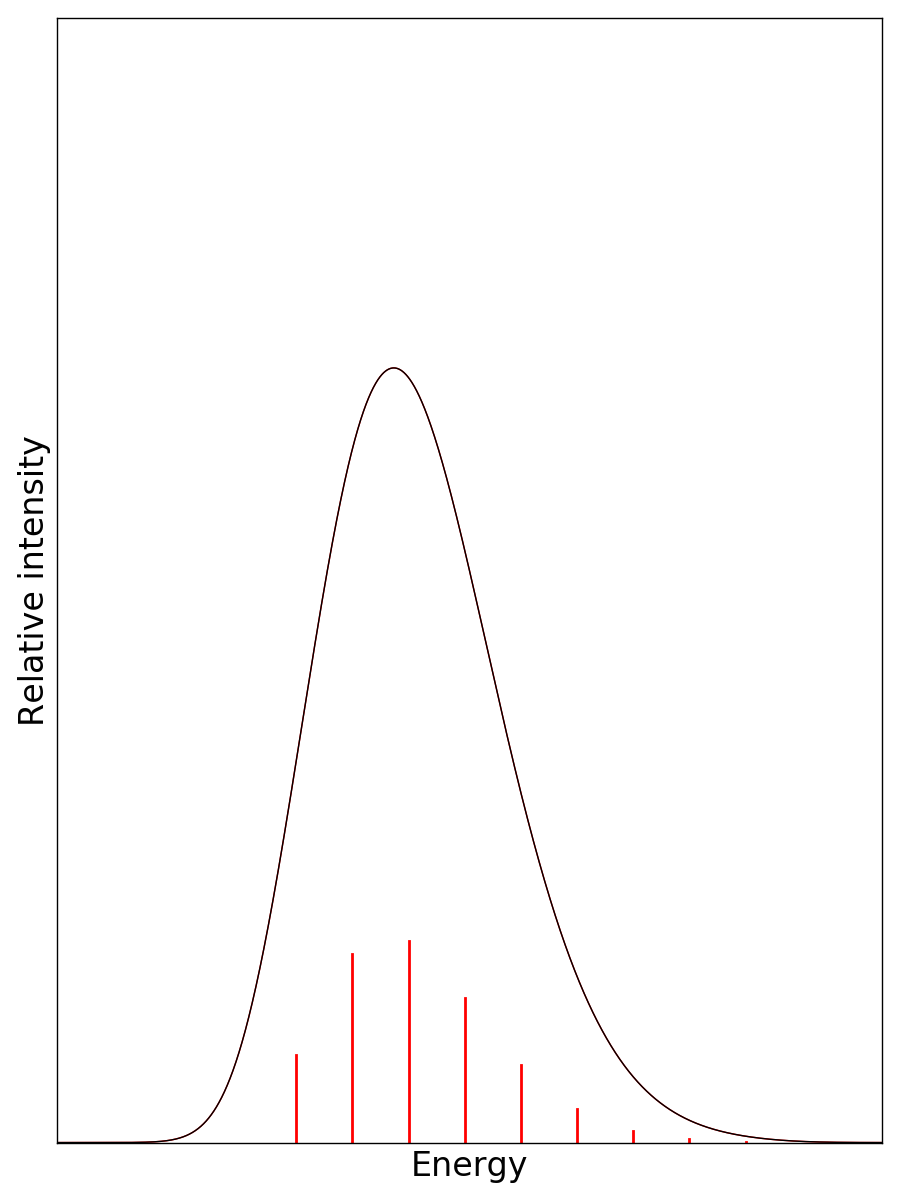
\includegraphics[width=\linewidth]{fc_sp/sp_8.png}
                \end{subfigure}
                %\caption{}
            \end{figure}
        }

    \end{overlayarea}
\end{frame}

\begin{frame}
    \frametitle{Generalization to N atoms}
    3N vibrational modes
    \pause
    \begin{align}
        d \to (d_1, d_2,... d_{3N}),  n &\to (n_1, n_2,... n_{3N}), \nonumber \\
        \mu \to (\mu_1, \mu_2,... \mu_{3N}), f &\to (f_1, f_2,... f_{3N}) \nonumber
    \end{align}
    \pause
    Irrelevant modes are dropped out \\
    $\to  2 \leq p \leq 10$ relevant modes
    \pause
    \begin{align}
        \mathrm{I}(n, n') &= \prod_{i=1}^{p} \;
        {\overbrace{\textstyle \mathrm{FCI}(n_i, n'_i)^2}^{\mathclap{\text{Overlap integral}}}} \;
        {\underbrace{\textstyle \exp\left( \frac{-\hbar n_i f_i}{k_B T} \right)}_{\mathclap{\text{Temperature term}}}} \nonumber 
    \end{align}
\end{frame}

\begin{frame}
    \frametitle{Calculating the integral}
    \begin{picture}(0, 0)
        \put(-5, 70){
            \begin{minipage}[t]{\linewidth}{
                Analytic solution when using harmonic potential
                \begin{align}
                    \mathrm{FCI}(n_i, n'_i)^2 &= e^{-S_i}S_i^{n'_i-n_I} \frac{n_i!}{n'_i!} \left[L_{n_i}^{n'_i-n_i}(S_i)\right]^2 \nonumber \\
                    S_i &= \frac{\delta_i^2 \mu_i f_i}{2 \hbar} \nonumber 
                \end{align}}
                If $S_i < S_{min}$ then mode $i$ is dropped out \\
                ~\\
                Values for $\delta, \mu$ and $f$ from AIMS
            \end{minipage}
        }
        \put(210, -120){
\includegraphics[height=4cm]{aims-2010-11-01_800x800.png}}
    \end{picture}

\end{frame}

\begin{frame}
    \frametitle{Transitions for Benzene}
    \begin{overlayarea}{\textwidth}{10cm}        
        \only<1>{
            \begin{wrapfigure}{r}{5.5cm}
                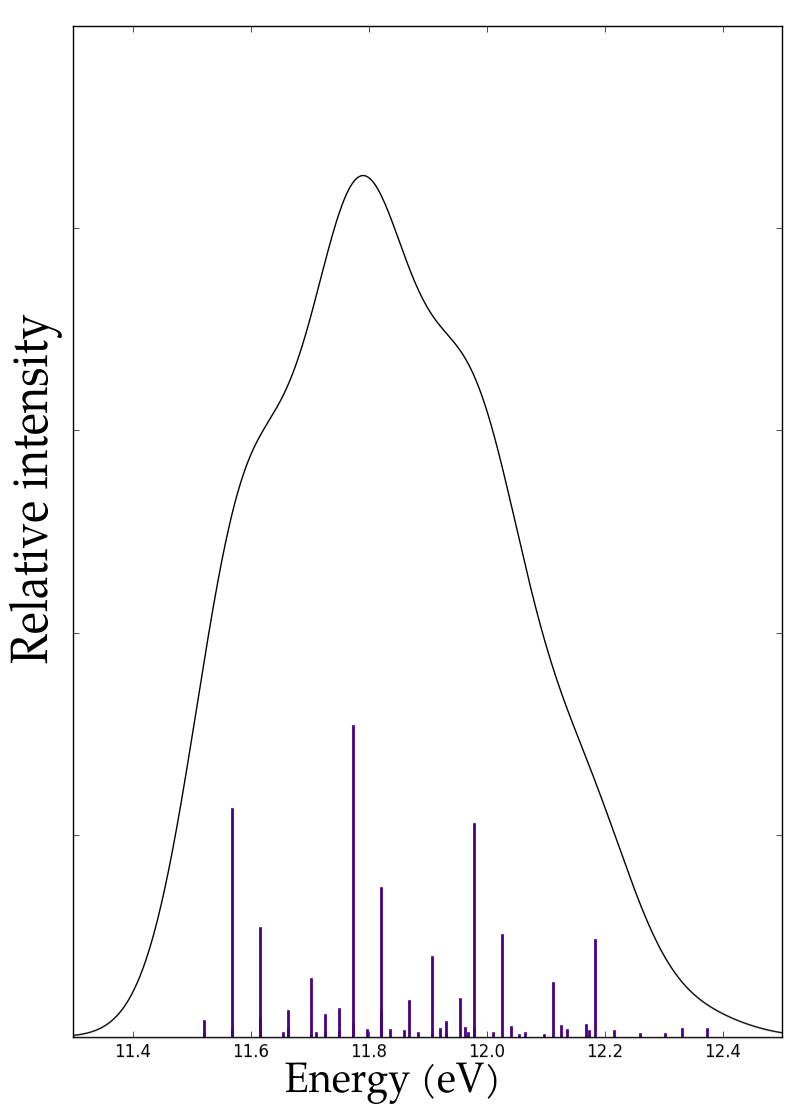
\includegraphics[width=5.5cm]{one_peak_1.png}
            \end{wrapfigure}
            ~\\
            More vibrational modes \\
            $\to$ more peaks
        }
        \only<2>{
            \begin{wrapfigure}{r}{5.5cm}
                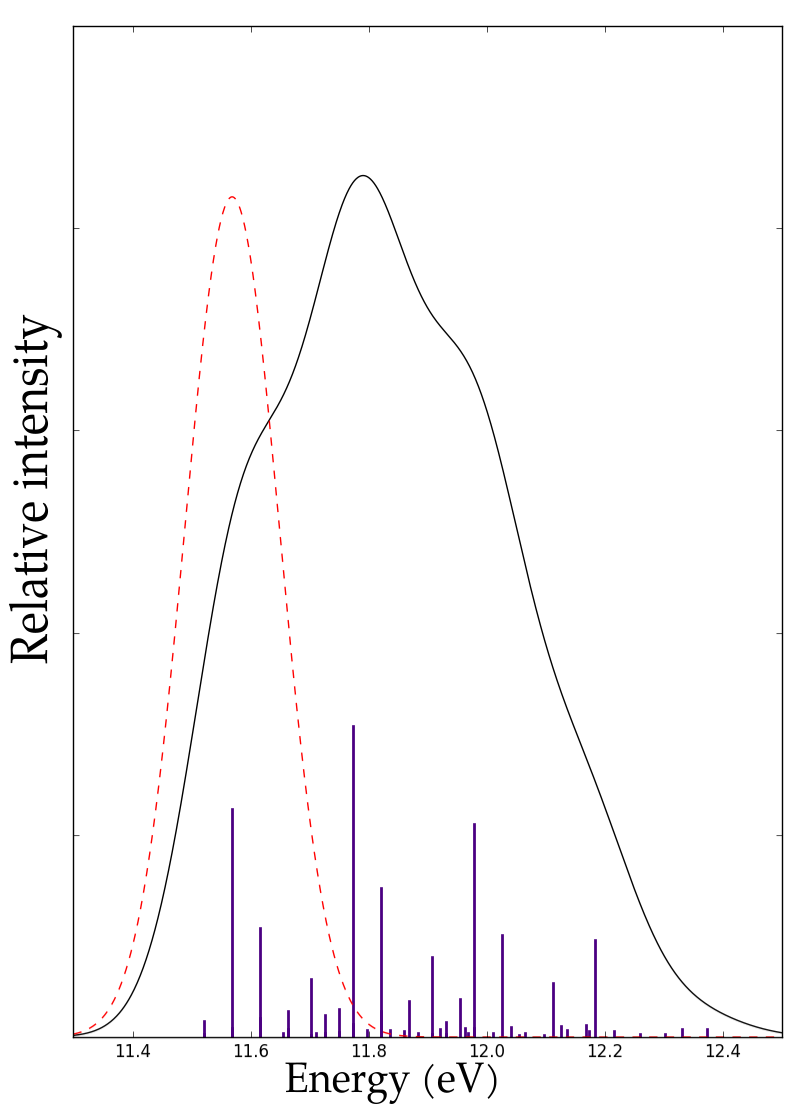
\includegraphics[width=5.5cm]{one_peak_2.png}
            \end{wrapfigure}
            ~\\
            More vibrational modes \\
            $\to$ more peaks \\
            ~\\
            Clear difference to the peak \\ without vibrations
            
        }
        \only<3>{
            \begin{wrapfigure}{r}{5.5cm}
                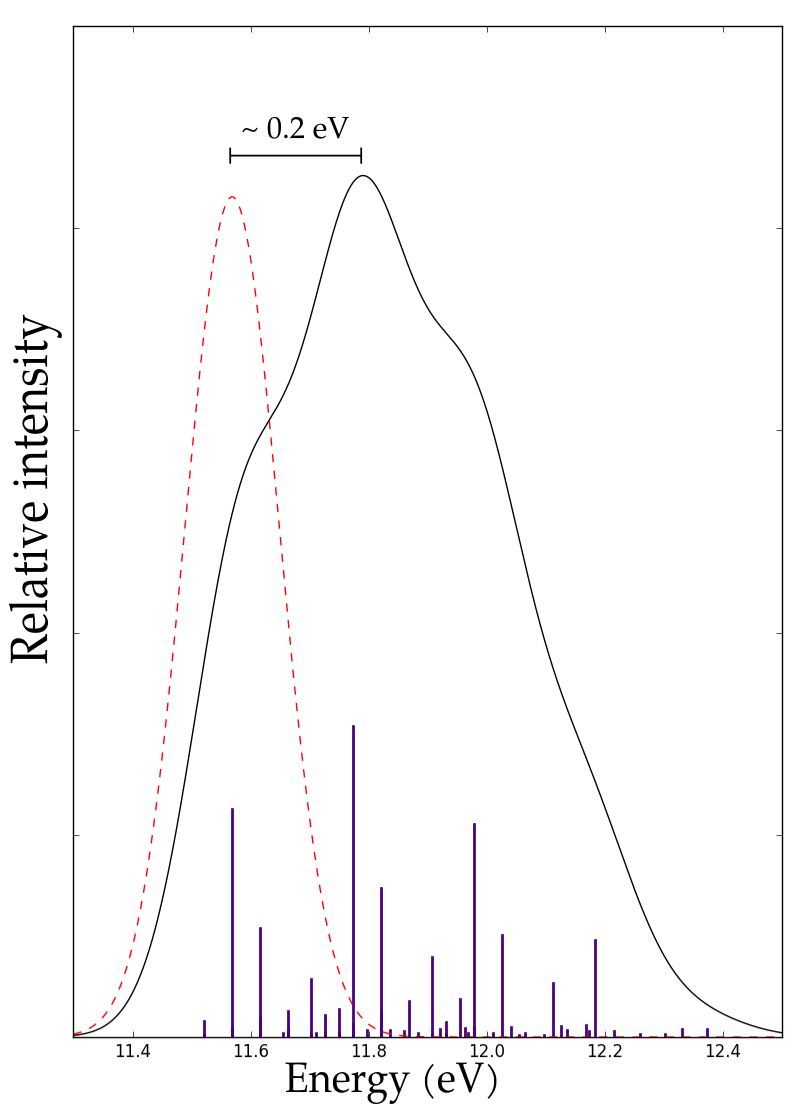
\includegraphics[width=5.5cm]{one_peak_3.png}
            \end{wrapfigure}
            ~\\
            More vibrational modes \\
            $\to$ more peaks \\
            ~\\
            Clear difference to the peak \\ without vibrations \\
            ~\\
            \mbox{Peaks shift from $0$ to $0.5 \ \mathrm{eV}$} \\
        }
        \only<4>{
            \begin{wrapfigure}{r}{5.5cm}
                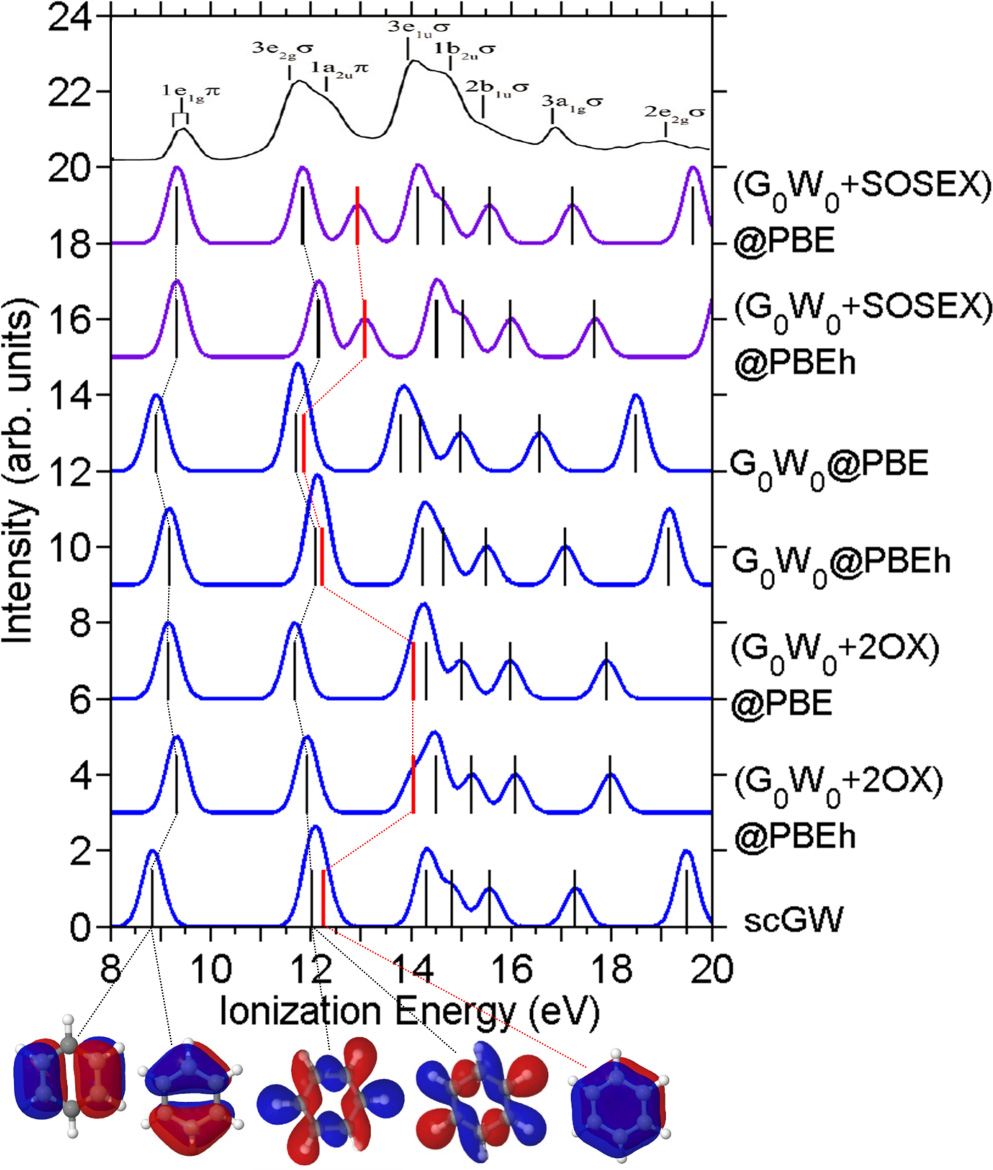
\includegraphics[width=5.5cm]{benzene_paper.png}
            \end{wrapfigure}
            ~\\
            More vibrational modes \\
            $\to$ more peaks \\
            ~\\
            Clear difference to the peak \\ without vibrations \\
            ~\\
            \mbox{Peaks shift from $0$ to $0.5 \ \mathrm{eV}$} \\
            ~\\
            Same order of magnitude as difference between theories
        }
    \end{overlayarea}
\end{frame}

\begin{frame}
    \frametitle{Peak shift}
    \begin{overlayarea}{\textwidth}{10cm}        
        \only<1>{
            \begin{figure}[h!]
                \caption*{Benzene}
                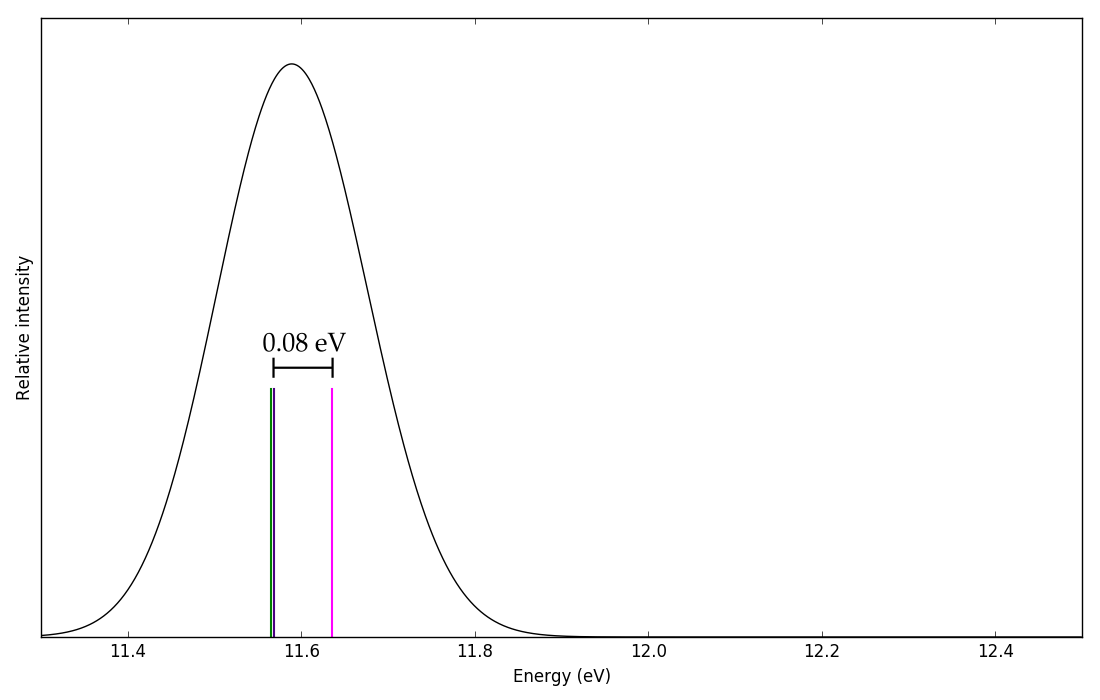
\includegraphics[width=\textwidth]{three_peaks_0.png}
            \end{figure}
        }
        \only<2>{
            \begin{figure}[h!]
                \caption*{Benzene}
                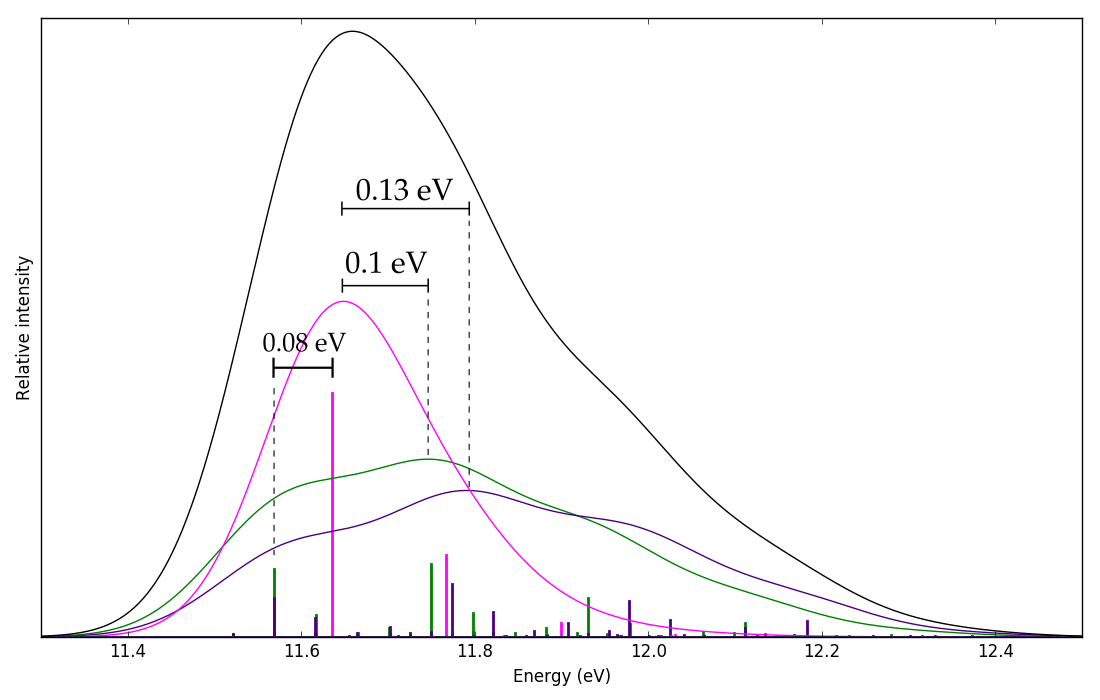
\includegraphics[width=\textwidth]{three_peaks_1.png}
            \end{figure}
        }
    \end{overlayarea}
\end{frame}

\begin{frame}
    \frametitle{Peak shift}
    \begin{overlayarea}{\textwidth}{10cm}        
        \only<1>{
            \begin{figure}[h!]
                \caption*{Ozone}
                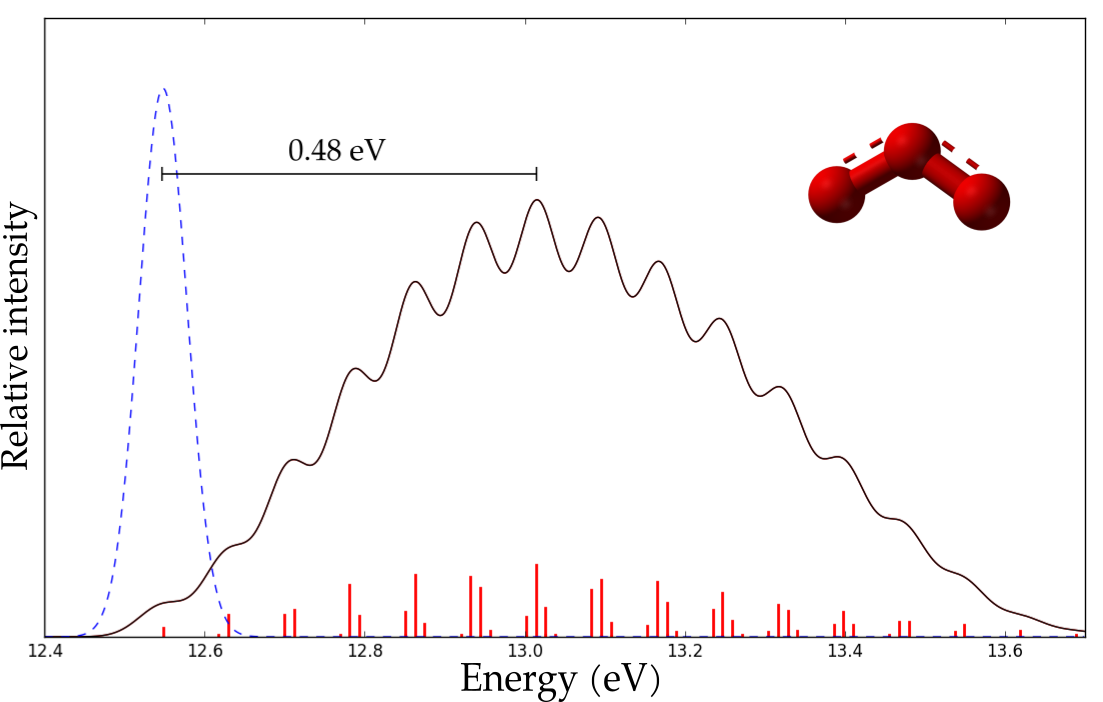
\includegraphics[width=\textwidth]{ozone.png}
            \end{figure}
        }
        \only<2>{
            \begin{figure}[h!]
                \caption*{Anthracene}
                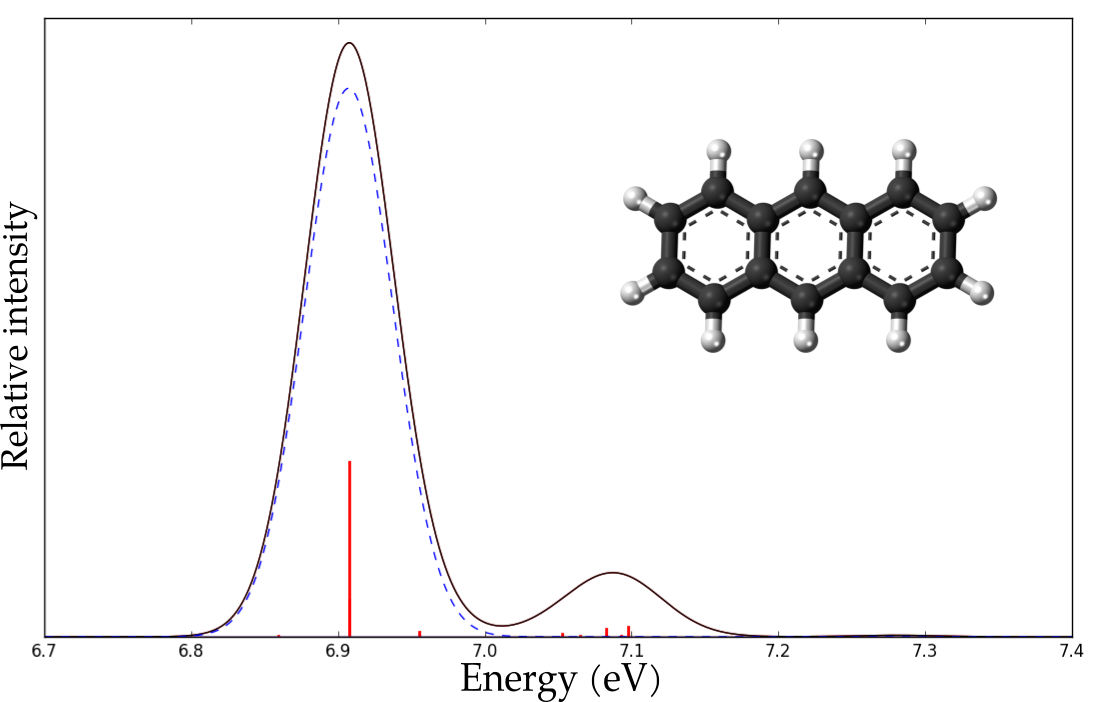
\includegraphics[width=\textwidth]{anthracene.png}
            \end{figure}
        }
    \end{overlayarea}
\end{frame}

\begin{frame}
    \begin{figure}
        \caption*{Benzene ionization spectra}
        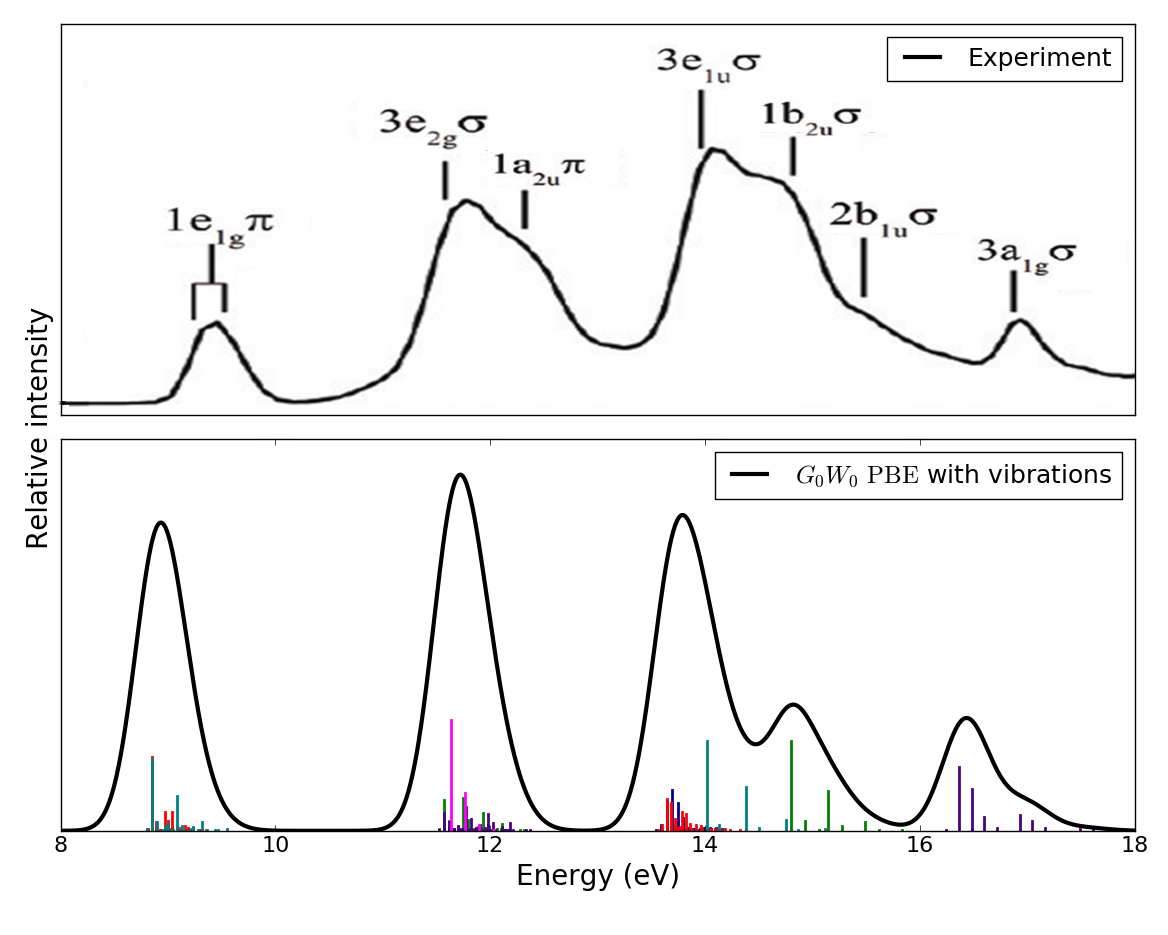
\includegraphics[width=0.9\textwidth]{all_peaks_thick.png}
    \end{figure}
\end{frame}

\begin{frame}
    \centering
    \begin{Large}
        Thank you! \\ ~\\
        Questions?
    \end{Large}
\end{frame}


\end{document}
